\documentclass[11pt,a4paper, twoside]{book}
\pagestyle{myheadings}
 
  
\usepackage[english]{babel}
\usepackage{graphicx}
\usepackage[colorlinks,hyperindex,plainpages=false]{hyperref}
\hypersetup{colorlinks=true,%
	linkcolor=black,%
	citecolor=red,%
	filecolor=blue,% 
	menucolor=black,%
	pagecolor=black,%
	urlcolor=black}
\usepackage{amssymb} 
\usepackage{wasysym}

\setlength{\parindent}{0pt} 
\setlength{\parskip}{0.3cm}

\title{
\flushright
{\LARGE\bfseries An Introduction to Metamodelling\\
and Graph Transformations}
\noindent\rule[-1ex]{\textwidth}{5pt}\\[2.5ex]
\hfill\emph{\LARGE\bfseries with eMoflon}
\flushleft
{\small Version 2.1}
\flushright

\includegraphics[width=0.85\textwidth]{pics/eMoflon3} 
}

\date{}  
\author{}  

\begin{document}  

\frontmatter 

\maketitle

\begin{small} 
  Copyright \copyright 2011--2012 Anthony Anjorin and Contributors. All rights
  reserved.

  This document is free; you can redistribute it and/or modify it
  under the terms of the GNU General Public License as published by
  the Free Software Foundation; either version 2 of the License, or
  (at your option) any later version.
 
  This document is distributed in the hope that it will be useful, but
  \emph{without any warranty}; without even the implied warranty of
  \emph{merchantability} or \emph{fitness for a particular purpose}.
  See the GNU General Public License for more details.
 
  You should have received a copy of the GNU General Public License
  along with this document; if not, write to the Free Software
  Foundation, Inc., 675 Mass Ave, Cambridge, MA 02139, USA.
\end{small}


\tableofcontents

\mainmatter

\section{Introduction}
testt
tset
\chapter{Installation}
\label{chap:installation}

\section{Install Our Plugin for Enterprise Architect (EA)}
Enterprise Architect (EA) is a modelling tool that supports
UML\footnote{Unified Modelling Language} and a host of other modelling
languages.  EA is not only affordable but is also quite flexible and can be
extended via \emph{plugins} to support new modelling languages.
\vspace{-0.1cm}
\begin{enumerate}
\item[$\blacktriangleright$] Download and install EA
(Fig.~\ref{fig_enterpriseArchitextHomepage})
\item[] Go to \url{http://www.sparxsystems.com.au/} to get a free 30 day trial.
\begin{figure}[!h]
	\centering
  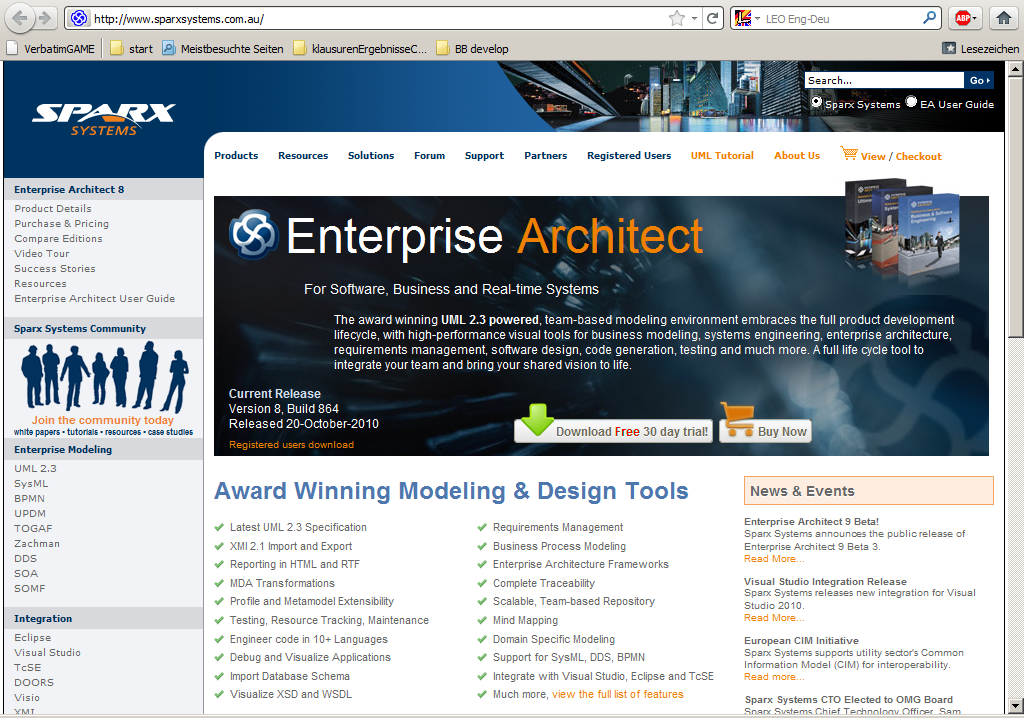
\includegraphics[width=0.7\textwidth]{pics/ea_download.png}
	\caption{Download Enterprise Architect}
	\label{fig_enterpriseArchitextHomepage}
\end{figure} 

\newpage

\item[$\blacktriangleright$] Install our EA-Plugin (Fig.~
\ref{fig_eaPluginWizard}) to add support for our modelling languages.
\item[] Download
\url{http://www.moflon.org/fileadmin/download/moflon-ide/eclipse-plugin/ea-ecore-addin/ea-ecore-addin.zip},
unpack, and run setup.exe
\begin{figure}[!h]
	\centering
  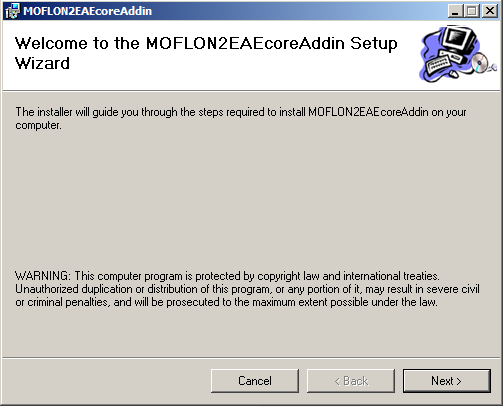
\includegraphics[width=0.3\textwidth]{pics/eaplugin_install.png}
	\caption{Install our plugin for EA.}
	\label{fig_eaPluginWizard}
\end{figure}
\end{enumerate}
\vspace{-1cm}

\section{Install Our Plugin for Eclipse}
\begin{enumerate}
\item[$\blacktriangleright$] Download and install Eclipse for Modeling
``Eclipse Modeling Tools (includes Incubating components)''
(Fig.~\ref{fig_downloadModelingPackage}) from:\\  
\url{http://www.eclipse.org/downloads/packages/}
\begin{figure}[!h]
	\centering
  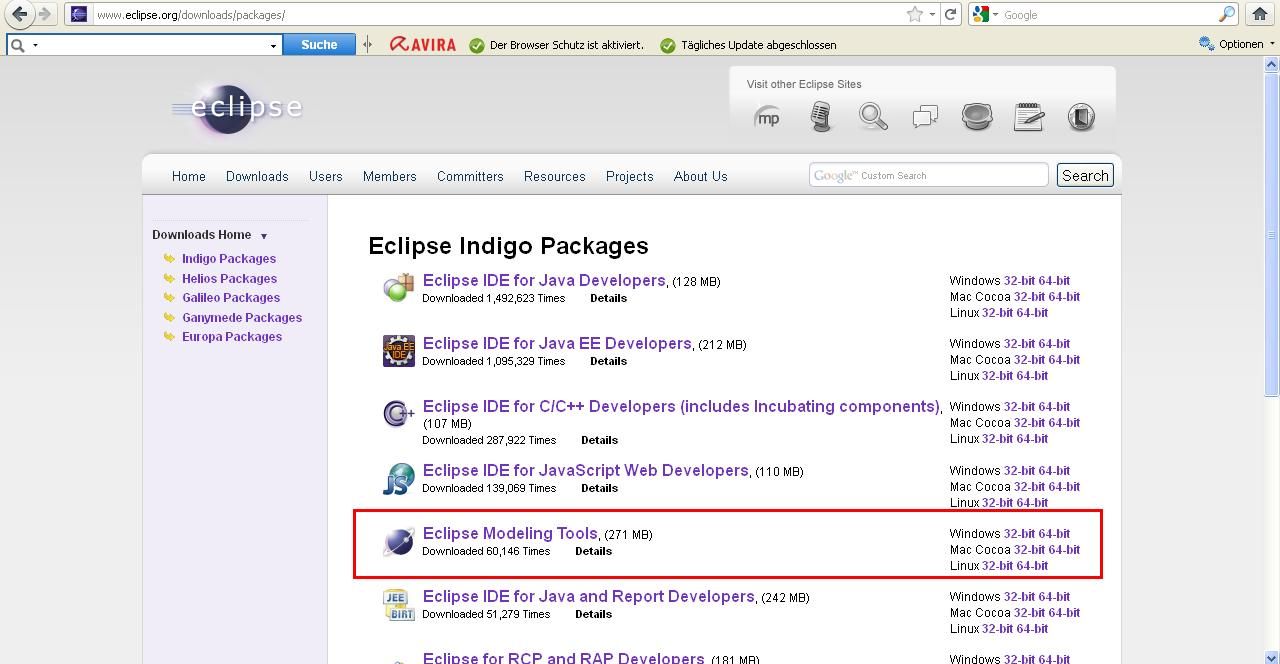
\includegraphics[width=0.7\textwidth]{pics/eclipse_modelingpackage.png}
	\caption{Download Eclipse Modeling Tools.}
	\label{fig_downloadModelingPackage}
\end{figure}
\vspace{-0.5cm}
\item[$\blacktriangleright$] Install our Eclipse Plugin from the following
update site\footnote{For a detailed tutorial on how to install Eclipse and
Eclipse Plugins please refer to
\url{http://www.vogella.de/articles/Eclipse/article.html}} 
\footnote{Please note: Calculating requirements and dependencies when installing
the plugin might take quite a while depending on your internet connection.}:
\url{http://www.moflon.org/fileadmin/download/moflon-ide/eclipse-plugin/update-site2}
\end{enumerate}

\section{Get a Simple Demo Running}

\begin{enumerate}
\item[$\blacktriangleright$] Go to ``Window/Open Perspective/Other\ldots'' and
choose Moflon (Fig.~\ref{fig_eclipse}).
\begin{figure}[!h]
	\centering
  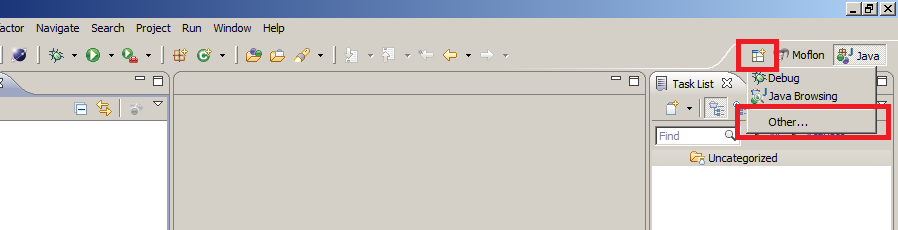
\includegraphics[width=0.7\textwidth]{pics/eclipse_firststart.png}
	\caption{Choose the Moflon Perspective.}
	\label{fig_eclipse}
\end{figure}

\item[$\blacktriangleright$] In the toolbar a new action set should have
appeared. Choose ``New Metamodel'' (Fig.~\ref{fig_eclipseNewMetamodel}).
The button with an ``L" shows you our logfile (important input for us if
something goes wrong!).
\begin{figure}[!h]
	\centering
  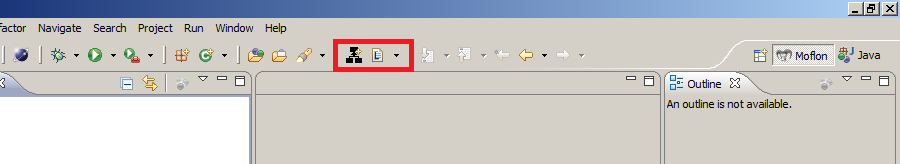
\includegraphics[width=0.8\textwidth]{pics/eclipse_metamodelButton.png}
	\caption{Eclipse New Metamodel}
	\label{fig_eclipseNewMetamodel}
\end{figure}

\item[$\blacktriangleright$] Enter ``Demo'' as the name of the new metamodel
project and confirm. 
An empty EA project file ``Demo.eap'' will be
created in a new project with a certain project structure
according to our conventions.

\newpage

\item[$\blacktriangleright$] Choose working sets as your top level element in
the package explorer (Fig.~\ref{fig_eclipseWorkingsets}).
We work a lot with working sets and use them to structure the workspace in
Eclipse.
\begin{figure}[!h]
	\centering
  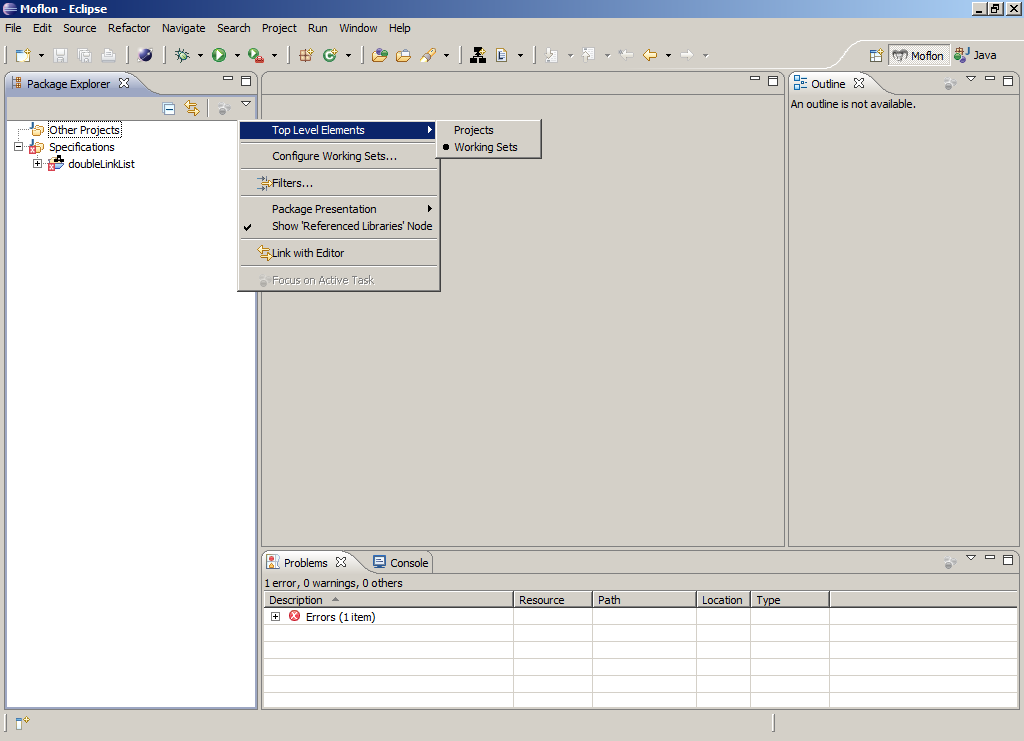
\includegraphics[width=0.6\textwidth]{pics/eclipse_workingsets.png}
	\caption{Choose Working Sets as Top Level Elements.}
	\label{fig_eclipseWorkingsets}
\end{figure}

\item[$\blacktriangleright$] Open the newly created project and replace the
``Demo.eap'' file with the Demo.eap that you will find in the
same folder as this tutorial. 
This EA file already contains our simple demo project.

\item[$\blacktriangleright$] Double click ``Demo.eap'' to start EA.
Please choose ``Ultimate" when starting EA for the first time.

\item[$\blacktriangleright$] In EA, choose ``Add-Ins/MOFLON::Ecore Addin/Export
all to Workspace'' (Fig.~\ref{fig_ea}).
\begin{figure}[!h]
	\centering
  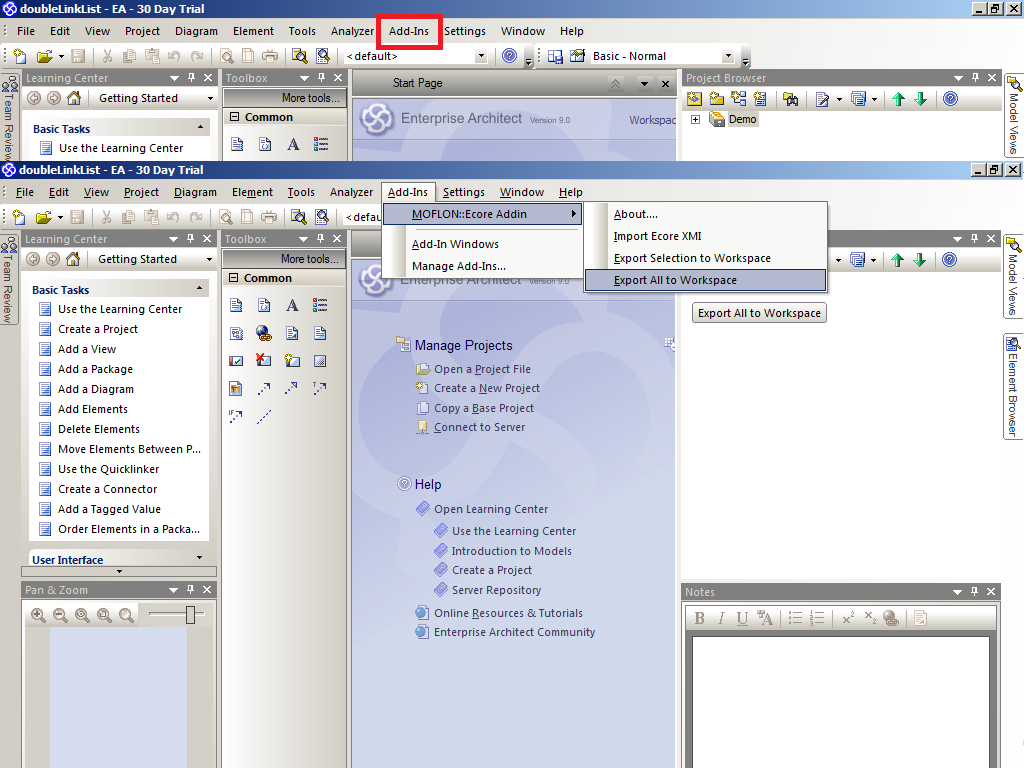
\includegraphics[width=0.65\textwidth]{pics/ea_firststart.png}
	\caption{Export from EA with our plugin.}
	\label{fig_ea}
\end{figure}

\newpage

\item[$\blacktriangleright$] Switch back to Eclipse, choose your Metamodel
project and press F5 to refresh.
The export from EA places all required files in a hidden folder in the
project, and refreshing triggers a build process that invokes our different
code generators automatically.
You should be able to monitor the progress in the lower right corner
(Fig.~\ref{fig_eclipsebuilding}).  
Pressing the symbol opens a monitor view that gives more details of the build
process. 
\begin{figure}[!h]
	\centering
  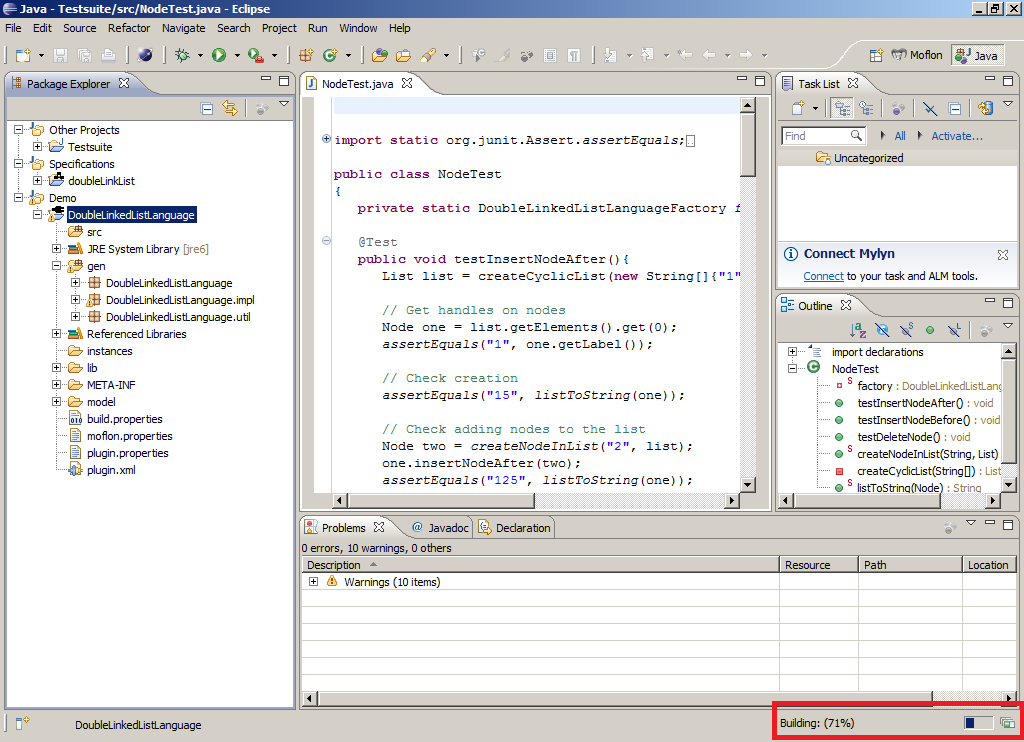
\includegraphics[width=0.6\textwidth]{pics/eclipse_building.png}
	\caption{Automatically building the workspace after a refresh.}
	\label{fig_eclipsebuilding}
\end{figure}
\end{enumerate}

\section{Validate Your Installation with JUnit}

\begin{enumerate}
\item[$\blacktriangleright$] Go to ``File/Import/General/Existing Projects
into Workspace'' (Fig.~\ref{fig_eclipseTestsuiteImport}) and choose the
Testsuite project that is also in the same folder as this tutorial. 
\begin{figure}[!h]
	\centering
  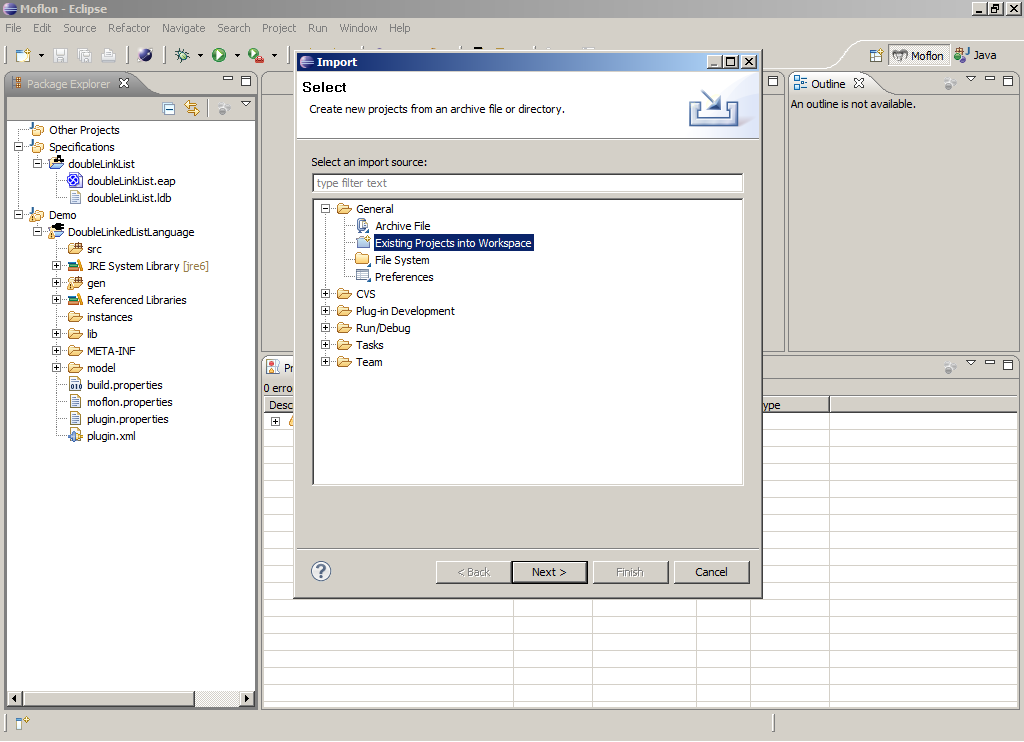
\includegraphics[width=0.6\textwidth]{pics/eclipse_testsuitimport.png}
	\caption{Import our Testsuite as an existing project.}
	\label{fig_eclipseTestsuiteImport}
\end{figure}

\newpage 

\item[] At this point, your workspace should resemble
Fig.~\ref{fig_eclipsepackageexplorer}.
\begin{figure}[!h]
	\centering
  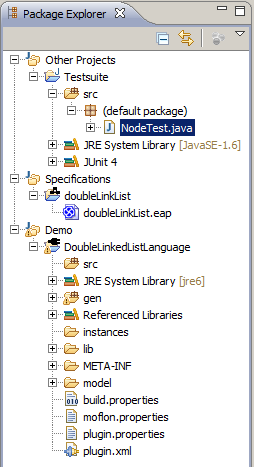
\includegraphics[width=0.2\textwidth]{pics/eclipse_packageexplorer.png}
	\caption{Workspace in Eclipse.}
	\label{fig_eclipsepackageexplorer}
\end{figure}

\item[$\blacktriangleright$] Right-click on the Testsuite project and select
``Run as/JUnit Test''.
Congratulations!  If you see a green bar  (Fig.~\ref{fig_eclipsetestsuiterun}),
then everything has been set-up correctly and you are now ready to start
metamodelling!
\begin{figure}[!h]
	\centering
  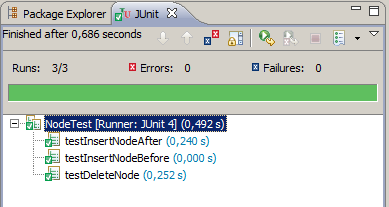
\includegraphics[width=0.2\textwidth]{pics/eclipse_testsuiterun.png}
	\caption{All's well that ends well\ldots}
	\label{fig_eclipsetestsuiterun}
\end{figure}
\end{enumerate}



\section{Project Structure and Setup}
Now that everything is installed and setup properly, let's take a closer look at
the different workspaces and workflow.  Before we continue, please make
a few slight adjustments to EA so you can easily compare your current workspace 
to our screenshots:
\begin{itemize}
  \item[$\blacktriangleright$] Select ``Tools/Options/Standard Colors'' in EA,
  and set your colours to reflect Fig.~\ref{fig_standardColoursEA}.
  \item[$\blacktriangleright$] In the same dialogue, select
  ``Diagram/Appearance'' and reflect the settings in
  Fig.~\ref{fig_standardAppearanceEA}.
  \item[$\blacktriangleright$] Last but not least, and still in the same
  dialogue, select ``Source Code Engineering'' and be sure to choose ``Ecore''
  as the default language for code generation (Fig.~\ref{fig_standardSCEEA}).
\end{itemize}
\newpage
%\usepackage{graphics} is needed for \includegraphics
\begin{figure}[!h]
\centering
\begin{minipage}[b]{0.3\textheight}
  \centering
  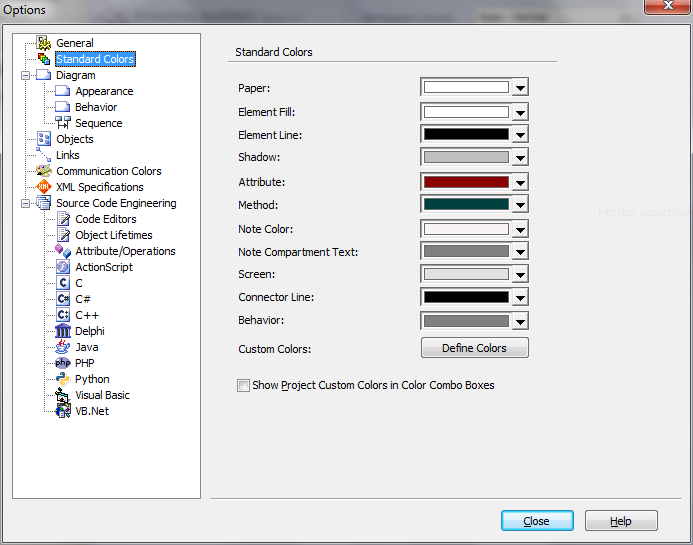
\includegraphics[width=\textwidth]{pics/standardColours}
  \caption{Our choice of standard colours for diagrams in EA.}
  \label{fig_standardColoursEA}
\end{minipage}
\\
\vspace{0.5cm}
\begin{minipage}[b]{0.3\textheight}
  \centering
  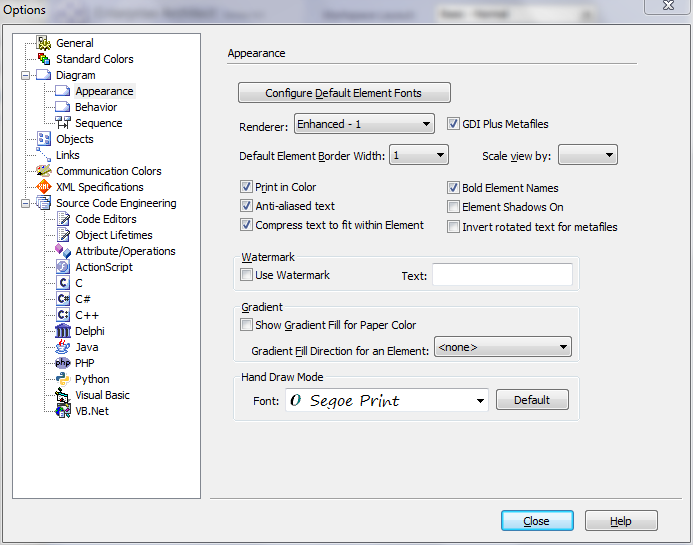
\includegraphics[width=\textwidth]{pics/standardAppearance}
  \caption{Our choice of the standard appearance for model elements in EA.}
  \label{fig_standardAppearanceEA}
\end{minipage}
\\
\vspace{0.5cm}
\begin{minipage}[b]{0.3\textheight}
  \centering
  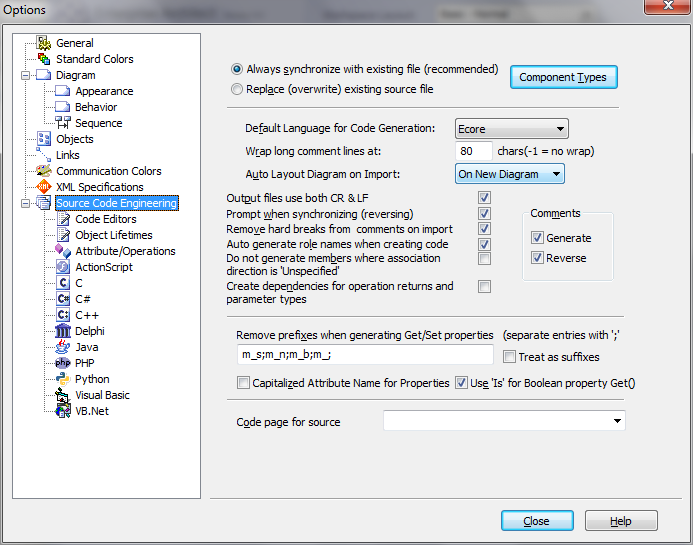
\includegraphics[width=\textwidth]{pics/standardCodeEngineering}
  \caption{Make sure you set the standard language to Ecore.}
  \label{fig_standardSCEEA}
\end{minipage}
\end{figure}

In your EA ``workspace'', actually referred to as an \emph{EA
project}\footnote{Words are set in italics when they represent concepts that are
introduced or defined  in the corresponding paragraph for the first time.}, take
a careful  look at the project structure:  The root node
\texttt{Demo}\footnote{Words set  in a \texttt{mono-space font} refer to things
that you should find in a tool,  dialogue, figure or code.} is called a
\emph{model} in EA lingo and is used as a  container to group a set of related
\emph{packages}. In our case, \texttt{Demo}  consists of a single package
\texttt{DoubleLinkedListLanguage}.  An EA project can however consist of
numerous models that in turn group  numerous packages.


Now switch to your \emph{Eclipse workspace} and note the two nodes named
\texttt{Spe\-ci\-fi\-ca\-tions} and \texttt{Demo}.  These nodes, used to group
related \emph{Eclipse projects} in an Eclipse workspace, are called
\emph{working sets}. The working set \texttt{Spe\-ci\-fi\-ca\-tions} contains
all \emph{metamodel projects} in a  workspace.
 A metamodel project contains a single EAP (EA project) file and is
used to communicate with EA and initiate codegeneration by simply pressing F5
or choosing ``refresh'' from the context menu.  In our case,
\texttt{Specifications} should contain a single metamodel project \texttt{Demo}
containing our EA project file  \texttt{Demo.eap}.

\begin{figure}[!h]
	\centering
  \includegraphics[width=0.8\textwidth]{pics/bothexplorers}
	\caption{From EA to Eclipse}
	\label{fig_fromEAtoEclipse}
\end{figure}

Figure~\ref{fig_fromEAtoEclipse} depicts how the Eclipse working set
\texttt{Demo} and its contents were generated from the EA model \texttt{Demo}.
Every model in EA is mapped to a working set in Eclipse with the same name. 
From every packages in the EA model, an Eclipse project is generated, also with
the same name.  These projects, however, are of a different
\emph{nature} than for example metamodel projects or normal Java projects, and
are called \emph{repository projects}.  A nature is Eclipse lingo for ``project
type'' and is visually indicated by a corresponding nature icon on the project
folder.  Our  metamodel projects sport a spanking little class diagram symbol. 
Repository projects are generated automatically  with a certain project
structure according to our conventions.  The  \texttt{model} subfolder is
probably most important, and contains an  \emph{Ecore model}.  Ecore is a
metamodelling language that provides building  blocks like \emph{classes} and
\emph{references} for defining the  static structure (concepts and relations
between concepts) of a system.  The  export function of our EA plugin generates
a valid Ecore model from the  corresponding EA model and persists it as an XML
file in the \texttt{model}  subfolder.  In our concrete example, this is the
\texttt{DoubleLinkedListLanguage.ecore} file.  Go ahead and double-click it to
open the file in a simple tree-view editor in Eclipse.  If you are really
interested in the nitty-gritty details or have a masochistic hang, right-click
the file and select ``Open With/Text Editor''. 

This Ecore model is used to drive a codegenerator that maps the model to Java
interfaces and classes.  The generated Java code that represents the model is
often referred to as a \emph{repository} and this is the reason why we refer to
such projects as repository projects.  A repository can be viewed as an
\emph{adapter} that enables building and manipulating concrete instances of a
specific model via a programming language like Java.  This is why we
indicate repository projects using a cute adapter/plug symbol on the project
folder.

Figure~\ref{fig_fromEAtoEclipse} depicts how the class \texttt{Node} in the EA
model is mapped to the Java interface \texttt{Node}.  Double-click
\texttt{Node.java} and take a look at the methods declared in the interface.
These correspond directly to the methods declared in the modelled \texttt{Node}
class.  Indicated by the source folders \texttt{src} and \texttt{gen}, we
advocate a clean separation of hand-written (this should go in \texttt{src}) and
generated code (lands automatically in \texttt{gen}).  As we shall see later in
the tutorial, hand-written code can also be integrated directly in generated
classes and, if marked appropriately, merged nicely by the codegenerator. 
This is sometimes more elegant for small helper functions but can quickly get
problematic especially in combination with source code management systems.

If you take a careful look at the code structure in \texttt{gen},
you'll find a \texttt{Foo\-Impl.java} for every \texttt{Foo.java}. Indeed, the 
subpackage \texttt{impl} contains Java classes that implement the interfaces in
the parent package.  Although this might strike you as unnecessary (why not
merge interface and implementation for simple classes?), this consequent
separation in interfaces and implementation allows for a clean and relatively
simple mapping of Ecore to Java, even in tricky cases like multiple inheritance
(allowed and very common in Ecore models).  A further package \texttt{util}
contains some auxiliary classes like a factory for creating instances of the
model.  If this is your first time of seeing generated code, you might be
shocked at the sheer amount of classes and code generated from our relatively
simple EA model.  You might be thinking: ``hey - if I did this by hand I
wouldn't need half of all this stuff!''.  Well you're right and you're wrong --
the point is that an automatic mapping to Java via a codegenerator scales quite
well.  This means for simple, trivial examples (like our double linked list), it
might be possible to come up with a leaner and simpler Java representation.  For
complex, large models with lots of mean pitfalls, however, this becomes a
daunting task.  The codegenerator provides you with years and years of
experience of professional programmers who have thought up clever ways
of handling multiple inheritance, an efficient event mechanism, reflection,
consistency between bidirectionally linked objects and much more.

A point to note here is that the mapping to Java is obviously not unique. 
Indeed there exist different standards of how to map a modelling language to a
general purpose programming language like Java.  We use a mapping defined and
implemented by the Eclipse Modelling Framework (EMF) which tends to favour
efficiency and simplicity.

Although getting the \emph{details} of mapping the static structure of our
models to Java might be extremely difficult, it seems for the most part pretty
straight  forward.  A fantastic productivity boost in any case but (yawn) not
exactly exciting.

Have you noticed the methods of the \texttt{Node} class in our EA model? 
Now hold on tight -- each method can be \emph{modelled} completely in EA and the
corresponding implementation in Java is generated automatically and placed in
\texttt{NodeImpl}.  Just in case you didn't get it: 
The behavioural or dynamic aspects of a system can be completely modelled in an
abstract, platform (programming language) independent fashion using a blend of
activity  diagrams and a ``graph pattern'' language called Story Driven
Modelling (SDM).  In our EA project, these ``Stories'', ``Story Models'' or
simply ``SDMs'' are  placed in SDM Containers named according to the method they
implement.  E.g.  \texttt{$\ll$ SDM Container$\gg$ insertNodeAfter SDM} for the
method  \texttt{insertNodeAfter(Node)} as depicted in
Fig.~\ref{fig_fromEAtoEclipse}.  We'll spend the rest of the tutorial
understanding why SDMs are so  {\huge crazily} cool!

\clearpage

To recap all we've discussed, let's consider the complete workflow as depicted
in Figure~\ref{fig_Overview}. We started with a concise model in EA, simple and
independent of any platform specific details (1).  Our EA model consists not
only of static aspects modelled as a class diagram (2), but also of dynamic
aspects modelled using SDM (3).  After exporting the model and codegeneration
(4), we basically switch from \emph{modelling}, to \emph{programming} in a
specific general purpose programming language (Java).  On this lower \emph{level
of abstraction}, we can flesh out the generated repository (5) if necessary, and 
mix as appropriate with hand-written code and libraries.  Our abstract specification of 
behaviour (methods) in SDM is translated to a series of method calls that form
the body of the corresponding Java method (6).
\begin{figure}[!h]
	\centering
  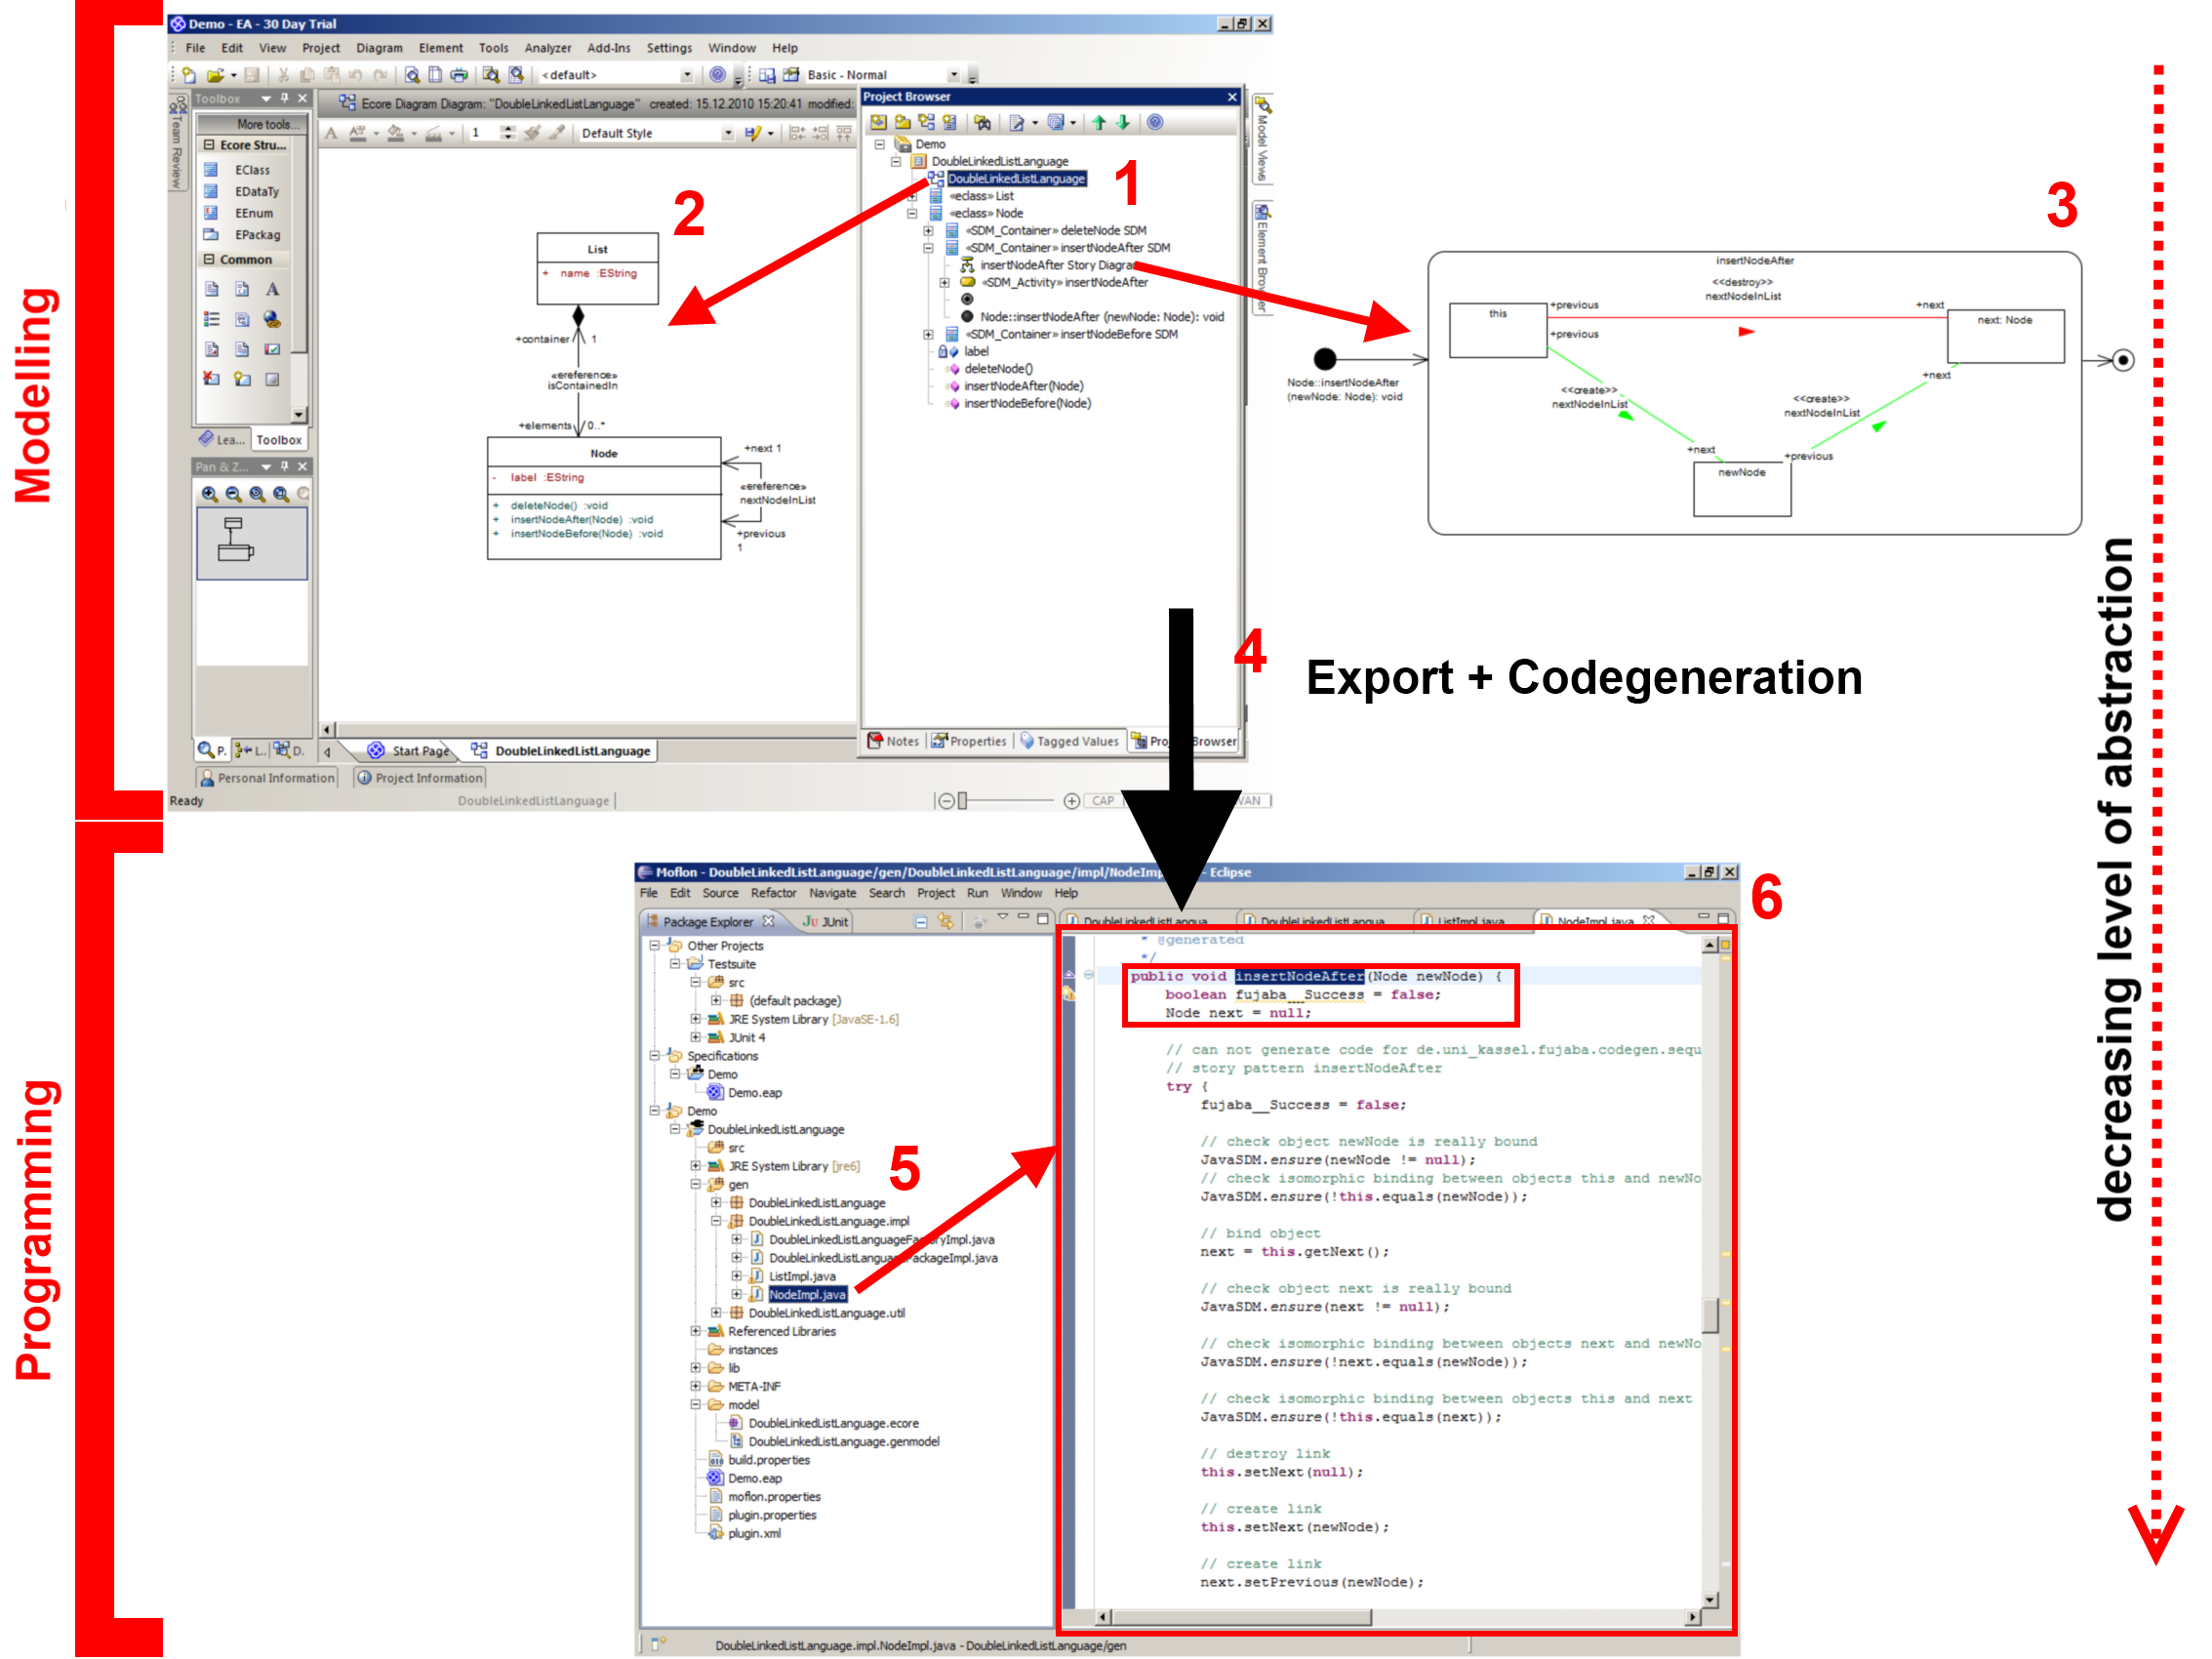
\includegraphics[width=1\textwidth]{pics/tafelbild}
	\caption{Overview}
	\label{fig_Overview}
\end{figure}


If you feel a bit lost at the moment please be patient, this first chapter has
been a lot about installation and tool support and only aims at giving a very
brief glimpse at the big picture of what is actually going on.    

In the following chapter, we shall go step-by-step through a hands-on example
and cover the core features of Ecore (static structure) and SDM (behaviour). 
We shall also give clear and simple definitions for the most important
metamodelling and graph transformation concepts, always referring to the
concrete example and providing lots of references for further reading.
\chapter{Modelling a Memory Box}
\label{chap:membox}

 The toughest part of learning a new language  is often building up a sufficient
vocabulary.  This is usually accomplished by repeating a long list of words
again and again till they stick.  A memory box is a simple but ingenious little
contraption to support this tedious process of memorisation.  As depicted in
Fig.~\ref{fig:membox_illustration}, it consists of a series of compartments or
partitions usually of increasing size.  The content to be memorised is written
on a series of cards  which are initially placed in the first partition.  All
cards in the first  partition should be repeated everyday and cards that have
been successfully  memorised are placed in the next partition.  Cards in all
other partitions are  only repeated when the corresponding partition is full and
cards that are  answered correctly are moved one partition forward in the box. 
Challenging  cards that have been forgotten are treated as brand new cards and
are always  placed right back into the first partition regardless of how far in
the box they  had progressed.  These ``rules'' are depicted by the green and red
arrows in  Fig.~\ref{fig:membox_illustration}. The basic idea is to repeat
difficult cards as often as necessary  and not to waste time on easy cards which
are only repeated now and then to keep them in memory.  The  increasing size of
the partitions represents how words are easily placed in our limited short term
memory and slowly move in our theoretically unlimited long term memory if
practised often enough.

%\usepackage{graphics} is needed for \includegraphics
\begin{figure}[htp]
\begin{center}
  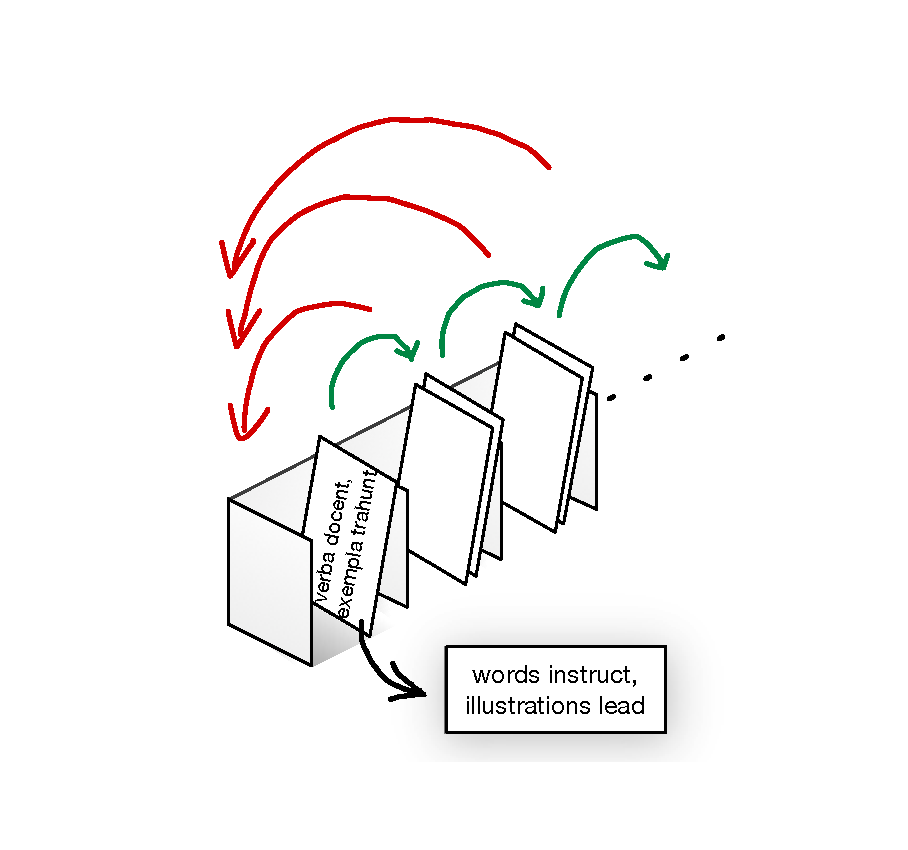
\includegraphics[width=0.4\textwidth]{pics/membox_illustration}
  \caption[]{Possible \emph{Concrete Syntax} of our Memory Box.}
  \label{fig:membox_illustration}
\end{center}
\end{figure}

A memory box is an interesting system, because it consists clearly of a static
structure (the box, partitions and their sizes, cards with their sides and
corresponding content) and a set of rules that describe the dynamic aspects 
(behaviour) of the system.  In the rest of the tutorial we shall build a
complete memory box from scratch in a model-driven fashion and use it to
introduce fundamental concepts in metamodelling and MDSD in general.  

\section*{A Language Definition Problem?}

Like in any area of study, metamodelling has its fair share of buzz words used
by experts to communicate concisely.  Although some concepts might seem quite
abstract for a beginner, a well defined vocabulary is important so we know
exactly what we are talking about.   

The first step is understanding that metamodelling equates to language
definition.  This means that the task of building a system like our memory box
can be viewed as defining a suitable language that can be used to describe the
system.  This language oriented approach has a lot of advantages including a
natural support for product lines (individual products are valid members of the
language) and a clear separation between platform independent and platform
specific details.      

So what constitutes a language?  The first question is obviously  how the
building blocks of your language actually ``look'' like.  Is your language to be
textual?  Visual?  This is referred to as the \emph{Concrete Syntax} of a
language and is basically an interface to end users who use the language.  
\marginpar{\emph{Concrete Syntax}}
In the case of our memory box, Fig.~\ref{fig:membox_illustration} can be viewed
as a possible concrete syntax.  As we are however building a memory box as a
software system, our actual concrete syntax  will probably be composed of GUI
elements like buttons, drop-down menus and text fields.   

Irrespective of how a language looks like, members of the language must adhere
to the same set of ``rules''.  
\marginpar{\emph{Grammar}}
For a natural language like English, this set of rules is usually called a
\emph{grammar}.  
In metamodelling, however, everything is represented as a graph of some kind
and, although the concept of a  \emph{graph grammar} is also quite well-spread
and understood, metamodellers  more often use a \emph{type graph} that defines
what types and relations  constitute a language. 
\marginpar{\emph{Graph Grammar}}
\marginpar{\emph{Type Graph}}
A graph that is a member of your language must \emph{conform to} the
corresponding type graph for the language.  To be more precise, it must be
possible to type the graph according to the type graph, i.e., the types and
relations used in the graph must exist in the type graph and not contradict the
structure defined there.  
\marginpar{\emph{Abstract Syntax}}
This way of defining membership to a language has many parallels to the
class-object relationship in the Object Oriented paradigm and should seem very
familiar for any programmer used to OO.  This type graph is referred to as the
\emph{Abstract Syntax} of a language. 

Very often, one might want to further constrain a language, beyond simple typing
rules.  
\marginpar{\emph{Static Semantics}}  
This can be accomplished with a further set of rules or constraints that
members of the language must fulfil in addition to being conform to the type
graph.
These further constraints are referred to as the \emph{Static Semantics}
of a language.    

With these few basic concepts, we can now introduce a further and central
concept in metamodelling, the \emph{metamodel} (basically a simple class
diagram). 
\marginpar{\emph{Metamodel}}
A metamodel defines not only the abstract syntax of a language but also some
basic constraints (a part of the static semantics).  
Thinking back to our memory box, we could define the types and relations we want
to allow, e.g.,  a box with partitions, cards, the box contains partitions that
contain cards. 
Multiplicities are an example for constraints that are no longer part of the
abstract syntax and belong to static semantics, but can nonetheless be expressed
in a metamodel.
For example, that a card can only be in one partition, or that a partition has
only one next partition or none.
\marginpar{\emph{Constraint Language}}  
More complex constraints that cannot be expressed in a metamodel are usually
specified using an extra \emph{constraint language} such as OCL (the Object
Constraint Language).
This goes beyond this tutorial however and we'll stick to metamodels without
using an extra constraint language.              

A short recap:  we have learnt that metamodelling starts with defining a
suitable language.  
For the moment, we know that a language comprises a concrete
syntax (how does the language look like),  an abstract syntax (types and
relations of the underlying graph structure), and static semantics (further
constraints that members of the language must fulfil).
\marginpar{\emph{Model}}
Metamodels are used to define the abstract syntax and a part of the static
semantics of a language, while \emph{models} are graphs that conform to some
metamodel (can be typed  according to the abstract syntax and adhere to the
static semantics). 

This tutorial is meant to be be hands-on so enough theory!  Lets
define, step-by-step, a metamodel for our memory box using our tool eMoflon.  
 
\section*{Abstract Syntax and Static Semantics with Ecore}

Switch to EA, choose \texttt{Demo} and click on the button \texttt{Add a
Package} as depicted in Fig.~\ref{fig:new_package}.   

\begin{figure}[htbp]
	\centering
  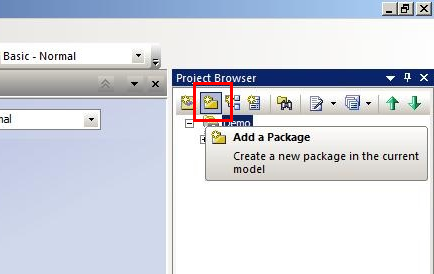
\includegraphics[width=0.5\textwidth]{pics/memBox01.png}
	\caption{Add a new package to \texttt{Demo}.}
	\label{fig:new_package}
\end{figure} 

In the dialogue that pops up (Fig.~\ref{fig:new_package_name}), choose
\texttt{Class View}, enter \texttt{Memory\-Box\-Language} as the name of the new
package and click \texttt{OK}. 

\begin{figure}[htbp]
	\centering
  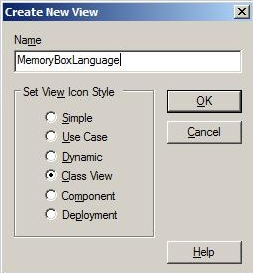
\includegraphics[width=0.3\textwidth]{pics/memBox02.png}
	\caption{Enter the name of the new package.}
	\label{fig:new_package_name}
\end{figure}

In your EA workspace the \texttt{Project Browser} should now look like
Fig.~\ref{fig:new_package_completed}.

\begin{figure}[htbp]
	\centering
  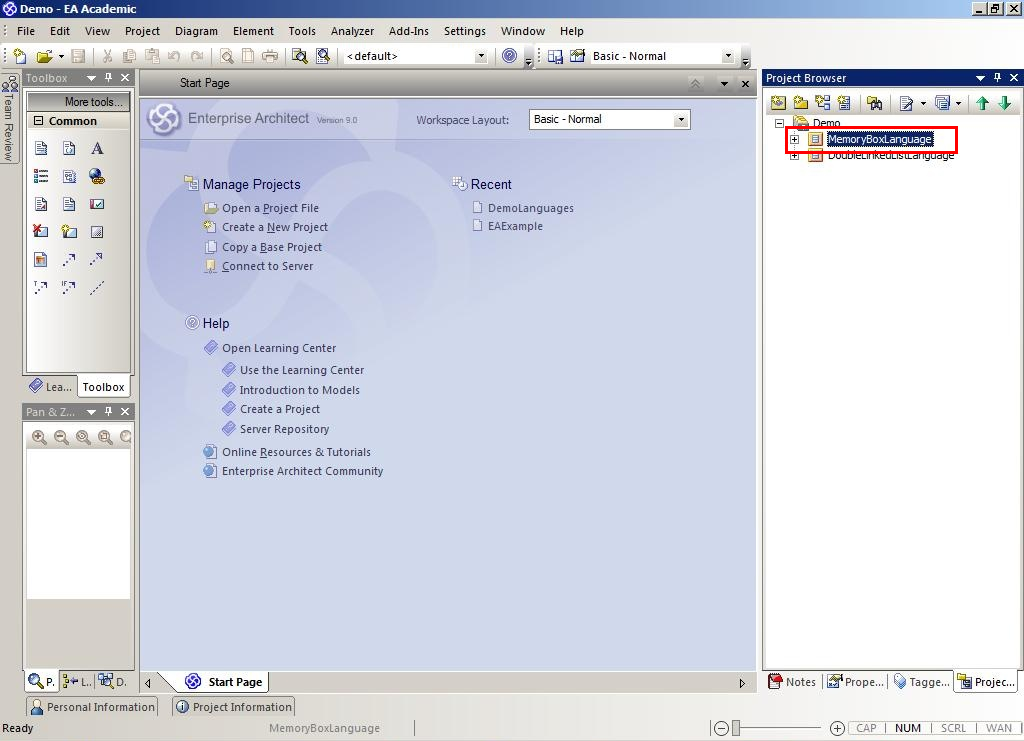
\includegraphics[width=0.5\textwidth]{pics/memBox03.png}
	\caption{State after creating the new package.}
	\label{fig:new_package_completed}
\end{figure}

\clearpage 

Now click the button \texttt{New Diagram} (Fig.~\ref{fig:diagram}).

\begin{figure}[htbp]
	\centering
  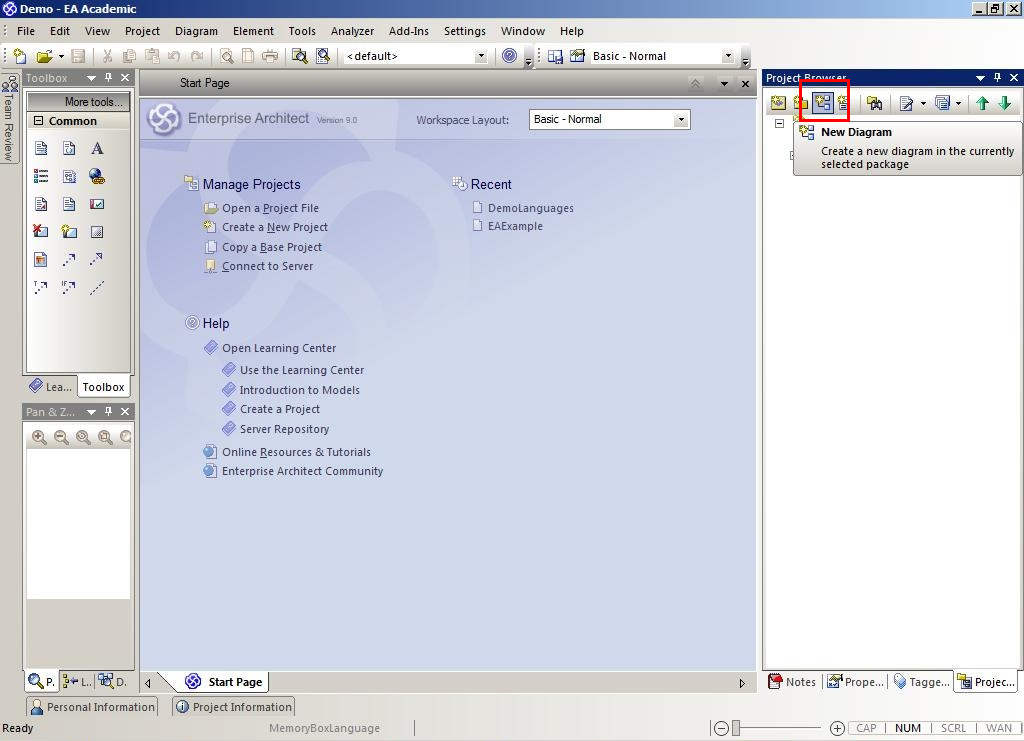
\includegraphics[width=0.7\textwidth]{pics/memBox04.png}
	\caption{Add a diagram.}
	\label{fig:diagram}
\end{figure}

In the dialog that pops up (Fig.~\ref{fig:diagram_type}), choose \texttt{Ecore
Diagram} and  \texttt{OK}. 


\begin{figure}[htbp]
	\centering
  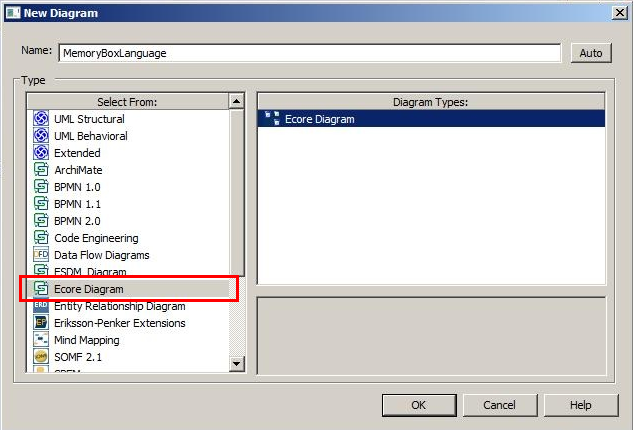
\includegraphics[width=0.8\textwidth]{pics/memBox05.png}
	\caption{Choose type of diagram.}
	\label{fig:diagram_type}
\end{figure}

In analogy to the ``everything is an object''
principle in the OO paradigm, in metamodelling, everything is a model.
\marginpar{\emph{Unification}}
This principle is called \emph{Unification} and has a lot of advantages.
If everything is a model, a metamodel that defines (at least a part of) a
language must be a model itself.
\marginpar{\emph{Meta-metamodel}}
\marginpar{\emph{Meta-Language}}
\marginpar{\emph{Modelling Language}}
This means that it conforms to some \emph{meta-metamodel} which defines a
\emph{(meta)modelling language} or \emph{meta-language}.
For metamodelling with eMoflon, we support \emph{Ecore} as a modelling language
and it defines types like \texttt{EClass} and \texttt{EReference}, which we will
be using to specify  our metamodels.
Other modelling languages include MOF, UML and Kermeta. 

\clearpage

After creating the new diagram, your  \texttt{Project Browser} should now
resemble Fig.~\ref{fig:diagram_completed}.  Double-click the newly
created diagram to ensure that it is open.

\begin{figure}[htbp]
	\centering
  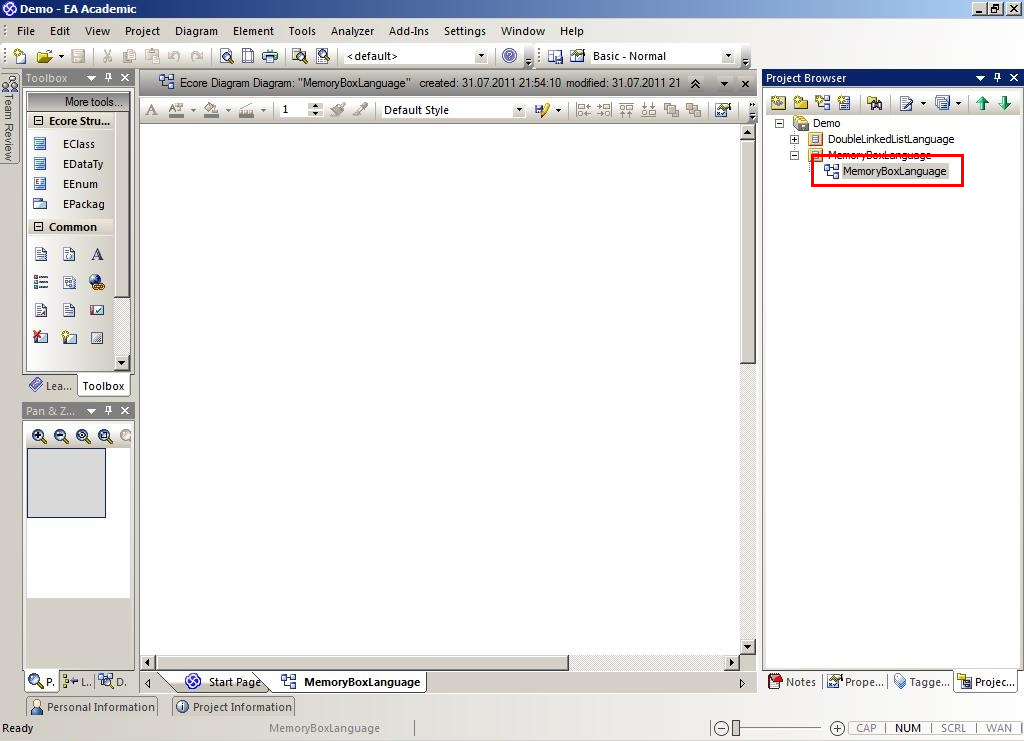
\includegraphics[width=0.7\textwidth]{pics/memBox06.png}
	\caption{State after creating diagram.}
	\label{fig:diagram_completed}
\end{figure}

To the left of the workbench in EA, a \emph{Toolbox} should have appeared
containing the types available in Ecore for metamodelling
(Fig.~\ref{fig:eclass}).  Click on \texttt{EClass} and click in the open
diagram (the main window in EA).

\begin{figure}[htbp]
	\centering
  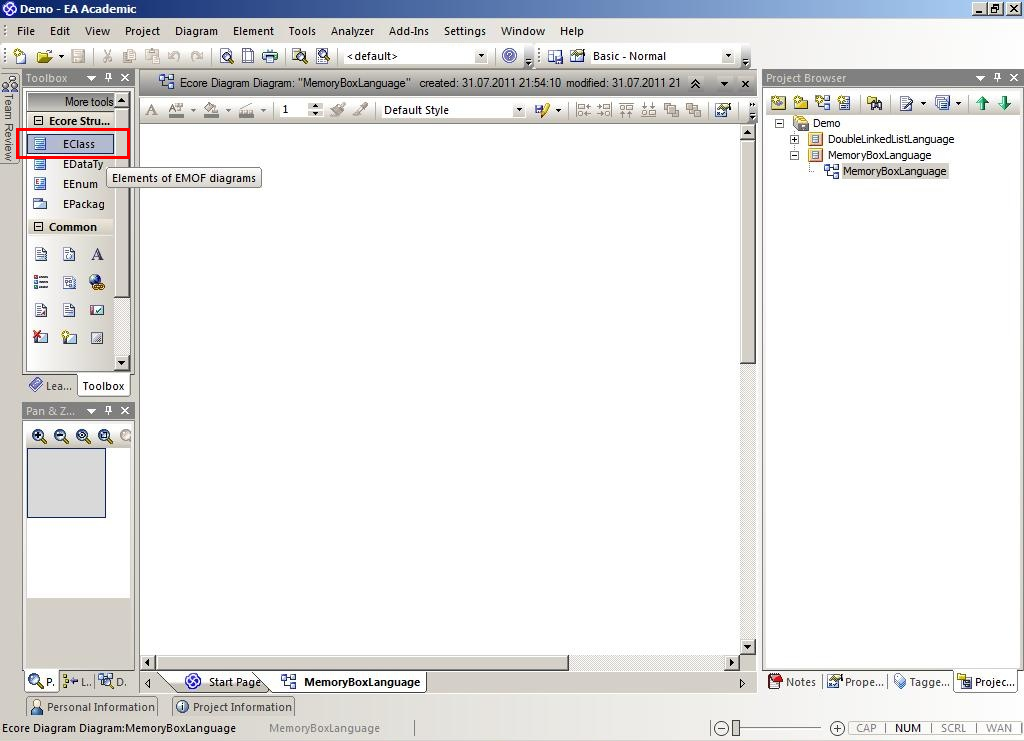
\includegraphics[width=0.7\textwidth]{pics/memBox07.png}
	\caption{Create an EClass.}
	\label{fig:eclass}
\end{figure}

\clearpage

In the dialogue that pops-up, enter \texttt{Box} as the name of the class and
click \texttt{OK} (Fig.~\ref{fig:eclass_properties}).  This dialogue can
always be invoked by double-clicking the class and contains many other
properties we'll be looking into later in the tutorial.  In general, a similar
``properties'' dialogue can be opened in the same fashion for almost every
element in EA.

\begin{figure}[htbp]
	\centering
  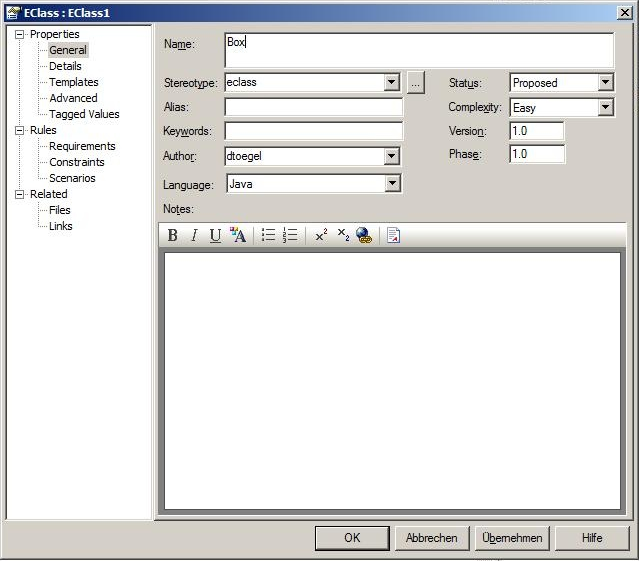
\includegraphics[width=0.6\textwidth]{pics/memBox08.png}
	\caption{Enter properties of EClass.}
	\label{fig:eclass_properties}
\end{figure}

After creating \texttt{Box}, your EA workspace should resemble
Fig.~\ref{fig:eclass_completed}. 

\begin{figure}[htbp]
	\centering
  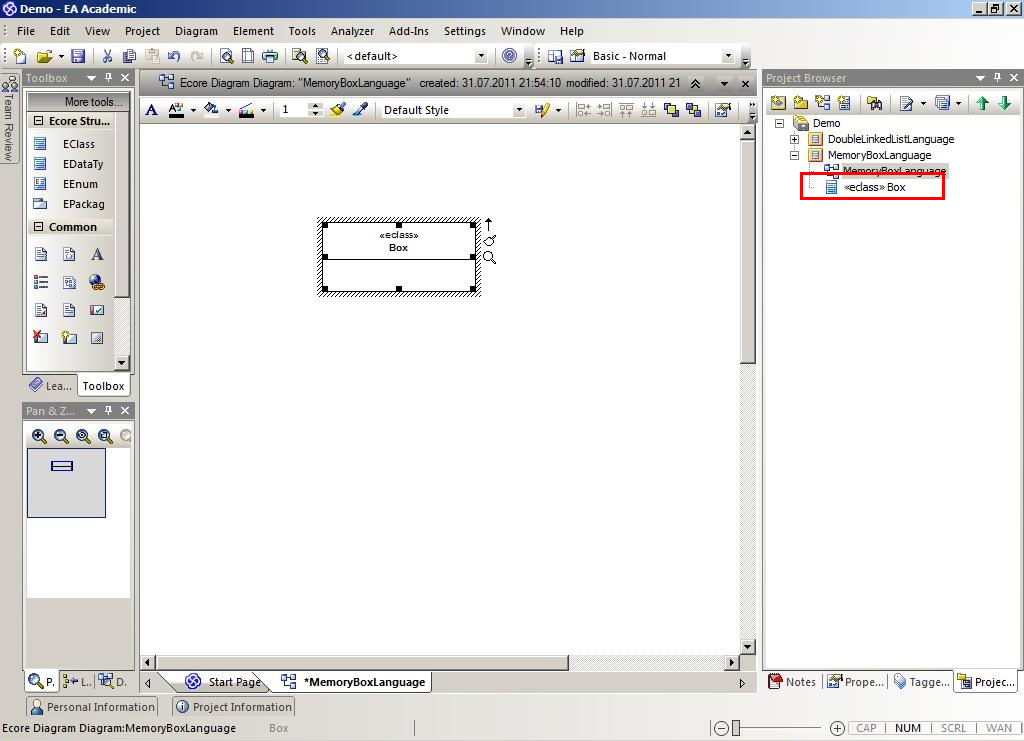
\includegraphics[width=0.7\textwidth]{pics/memBox09.png}
	\caption{State after creating \texttt{Box}.}
	\label{fig:eclass_completed}
\end{figure}

\clearpage

Now create \texttt{Partition} and \texttt{Card} in the same way, till your
workspace resembles Fig.~\ref{fig:all_eclasses}.  These are the main classes for
our memory box.

\begin{figure}[htbp]
	\centering
  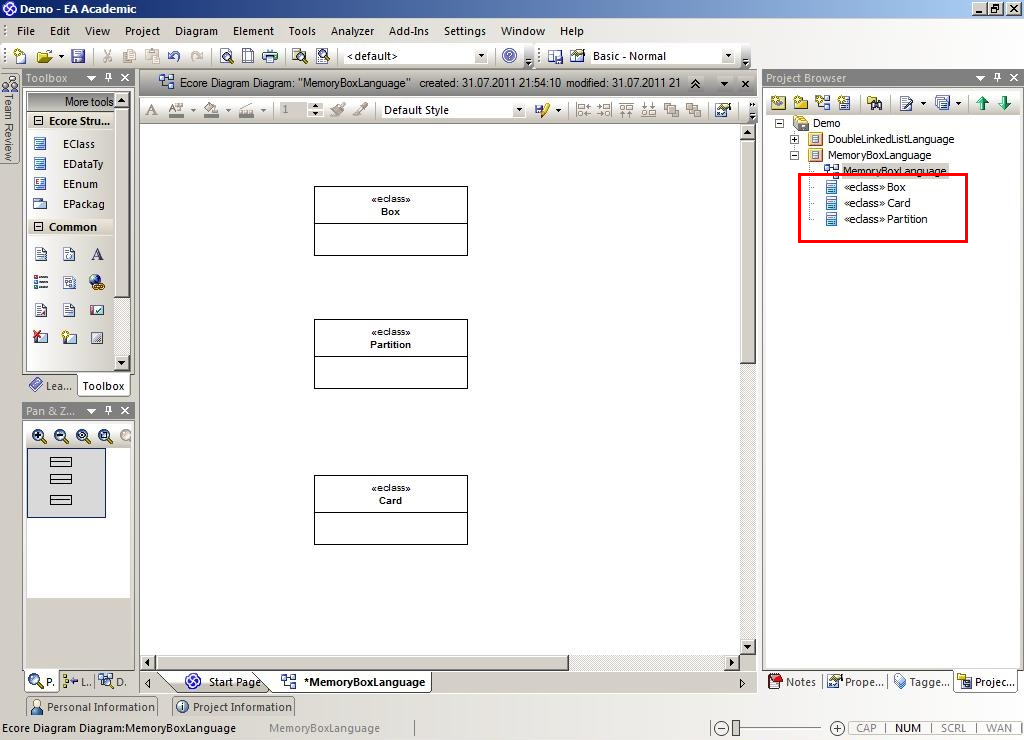
\includegraphics[width=0.7\textwidth]{pics/memBox10.png}
	\caption{Main classes in our metamodel.}
	\label{fig:all_eclasses}
\end{figure}

Now choose \texttt{Box}, right-click to call up the context menu and choose
\texttt{Att\-ri\-butes\ldots} (Fig.~\ref{fig:attribute}).

\begin{figure}[htbp]
	\centering
  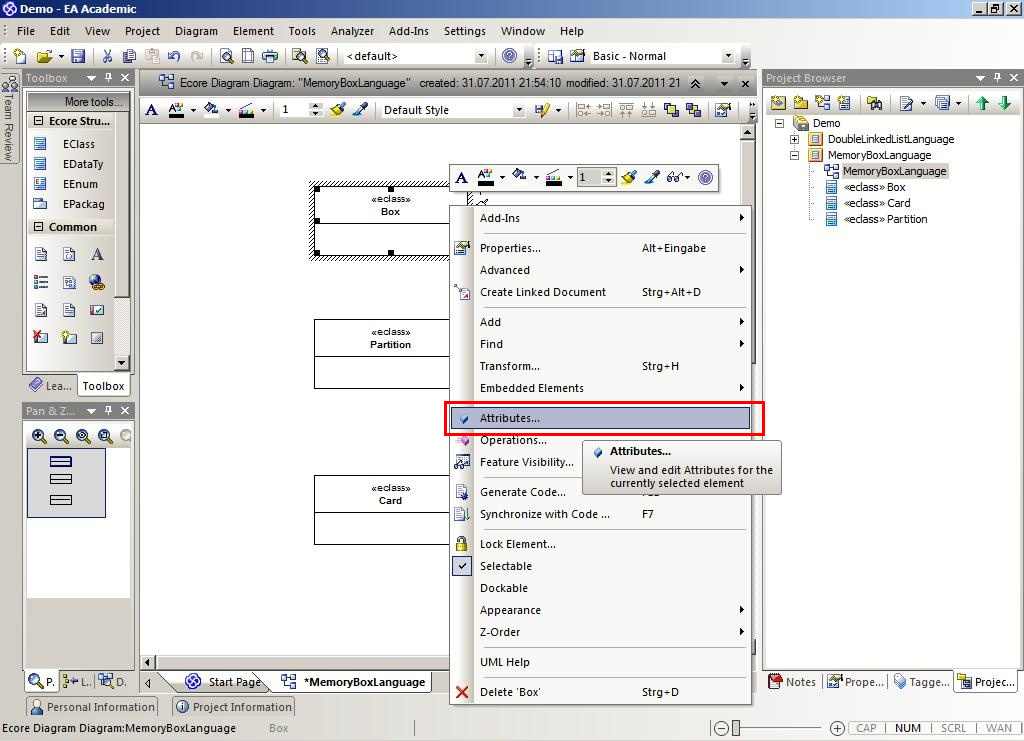
\includegraphics[width=0.7\textwidth]{pics/memBox11.png}
	\caption{Context Menu for a class.}
	\label{fig:attribute}
\end{figure}

\clearpage

In the dialogue that pops-up, enter \texttt{name} as the name of the attribute,
choose \texttt{EString} as its type and press \texttt{Save}
(Fig.~\ref{fig:attribute_properties}).  A new attribute for the same class can
be added by choosing \texttt{New}.

\begin{figure}[htbp]
	\centering
  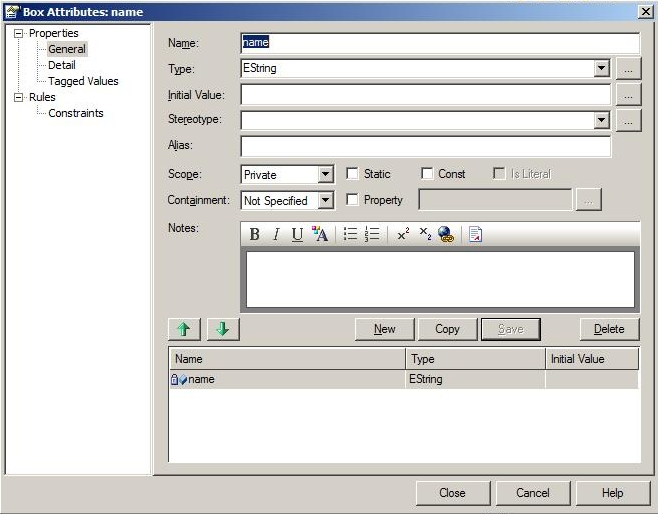
\includegraphics[width=0.7\textwidth]{pics/memBox13.png}
	\caption{Adding attributes to a class.}
	\label{fig:attribute_properties}
\end{figure} 

Add attributes to the other classes till your workspace resembles
Fig.~\ref{fig:attribute_completed}.

\begin{figure}[htbp]
	\centering
  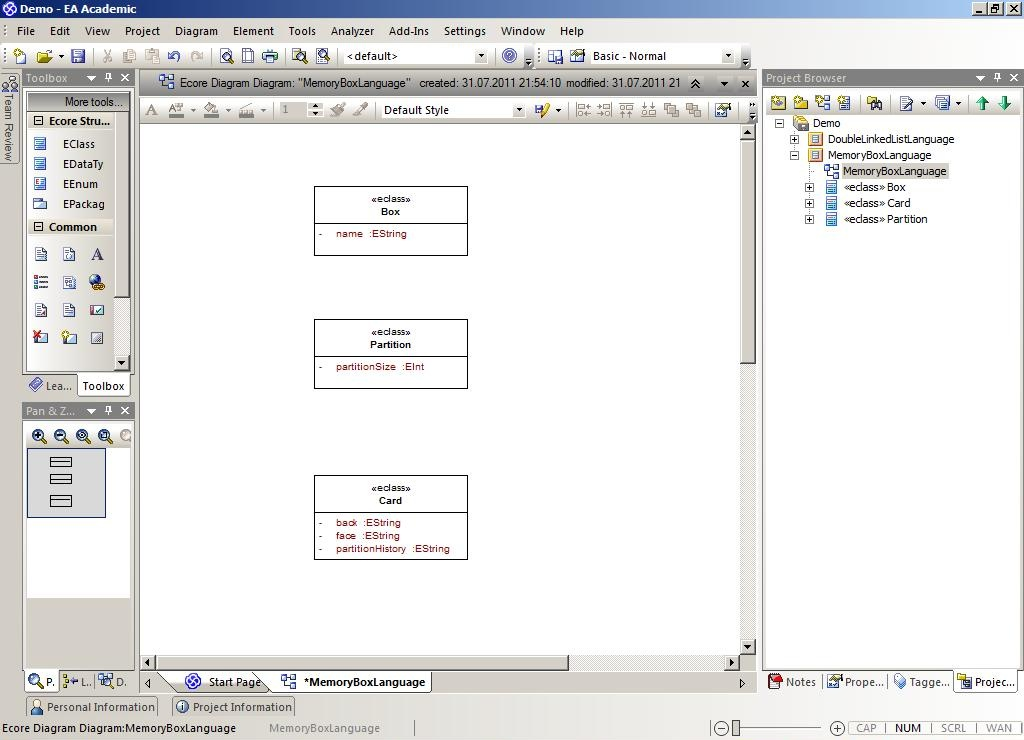
\includegraphics[width=0.73\textwidth]{pics/memBox14.png}
	\caption{Main classes with attributes.}
	\label{fig:attribute_completed}
\end{figure}

\clearpage

Now choose \texttt{EPackage} from the toolbox and add it to the current diagram
just like how we added EClasses. Enter \texttt{facade} as the name of the
package. 

Ecore supports packages that can be used to structure and group classes
in a metamodel.  In our case, we need  a util class that implements helper
methods for our memory box.  These methods  will be implemented by hand in Java
and the util class thus represents a kind of  interface or ``facade'' between
our model and hand-written code.  We shall soon  see how our Eclipse Plugin
offers extra support if one follows this naming  convention for packages
containing hand-written code. 

To add a class to our new package, select it in the Project Browser and then
press the button \texttt{Create Element} (Fig.~\ref{fig:epackage_newelement}).  

\begin{figure}[htbp]
	\centering
  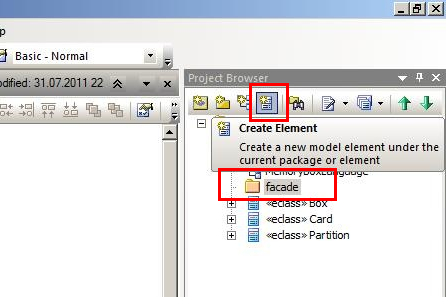
\includegraphics[width=0.6\textwidth]{pics/memBox19.png}
	\caption{Add a class to the package.}
	\label{fig:epackage_newelement}
\end{figure}

In the dialogue that pops-up, the correct toolbox should be preselected.  Enter
\texttt{MemoryBoxUtil} as the name of the class and click \texttt{Create}
(Fig.~\ref{fig:epackage_createelement}).

\begin{figure}[htbp]
	\centering
  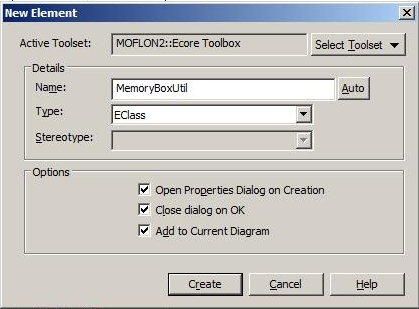
\includegraphics[width=0.5\textwidth]{pics/memBox20.png}
	\caption{Enter name of class to create.}
	\label{fig:epackage_createelement}
\end{figure}

\clearpage

Your workspace should now resemble Fig.~\ref{fig:epackage_completed}.  Every
subpackage like \texttt{facade} can also contain diagrams that can be created
and added using the Project Browser just like how we created the current
diagram. In this way an arbitrary nesting of packages is possible.

\begin{figure}[htbp]
	\centering
  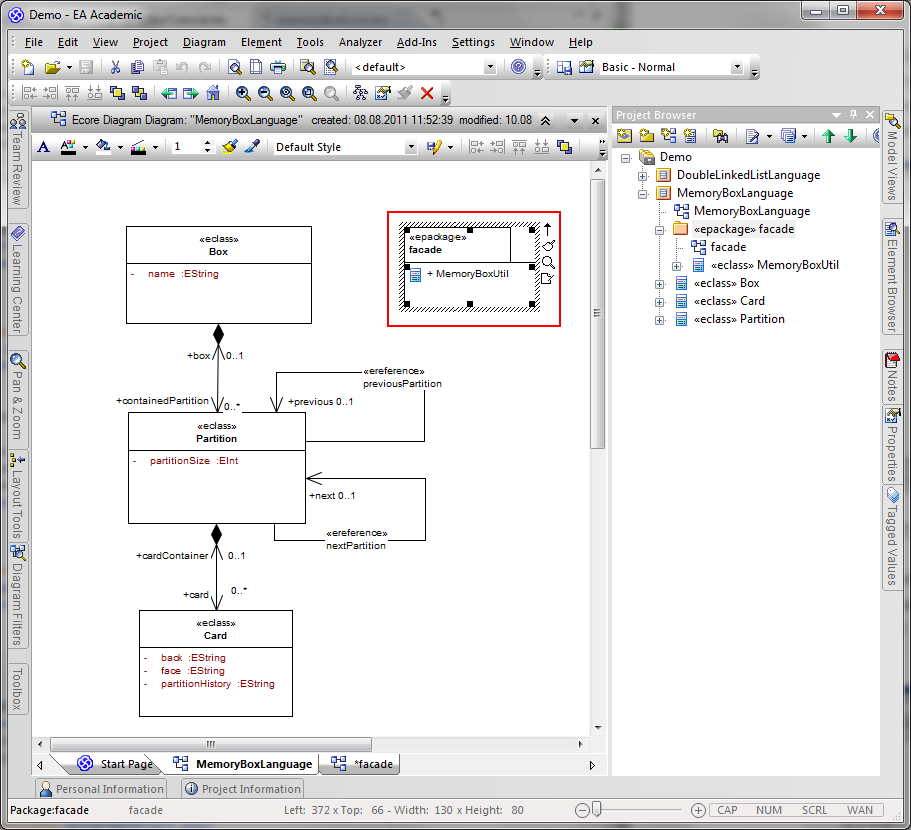
\includegraphics[width=0.7\textwidth]{pics/memBox22.png}
	\caption{Workspace after adding package.}
	\label{fig:epackage_completed}
\end{figure}

A fundamental gesture in EA is \emph{Quick Link}.  Quick Link is used to create
links between elements in a context sensitive manner.  To use Quick Link,
choose an element and note the little black arrow in its top-right corner
(Fig.~\ref{fig:quicklink}).

\begin{figure}[htbp]
	\centering
  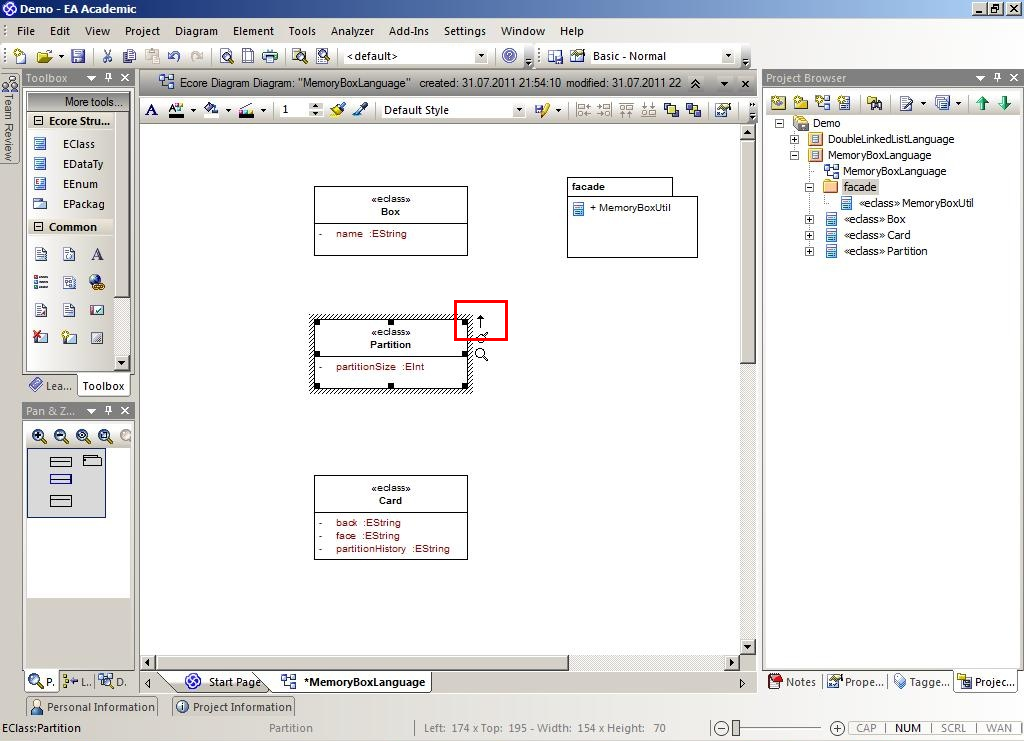
\includegraphics[width=0.7\textwidth]{pics/memBox23.png}
	\caption{Quick Link is a central gesture in EA.}
	\label{fig:quicklink}
\end{figure}

\clearpage

Now click on the black arrow and pull to another element you wish to ``quick
link" to.  In this case quick link from \texttt{Partition} to \texttt{Box}.  In
the context-menu that pops-up, choose \texttt{EReference}.
(Fig.~\ref{fig:ereference}). 

\begin{figure}[htbp]
	\centering
  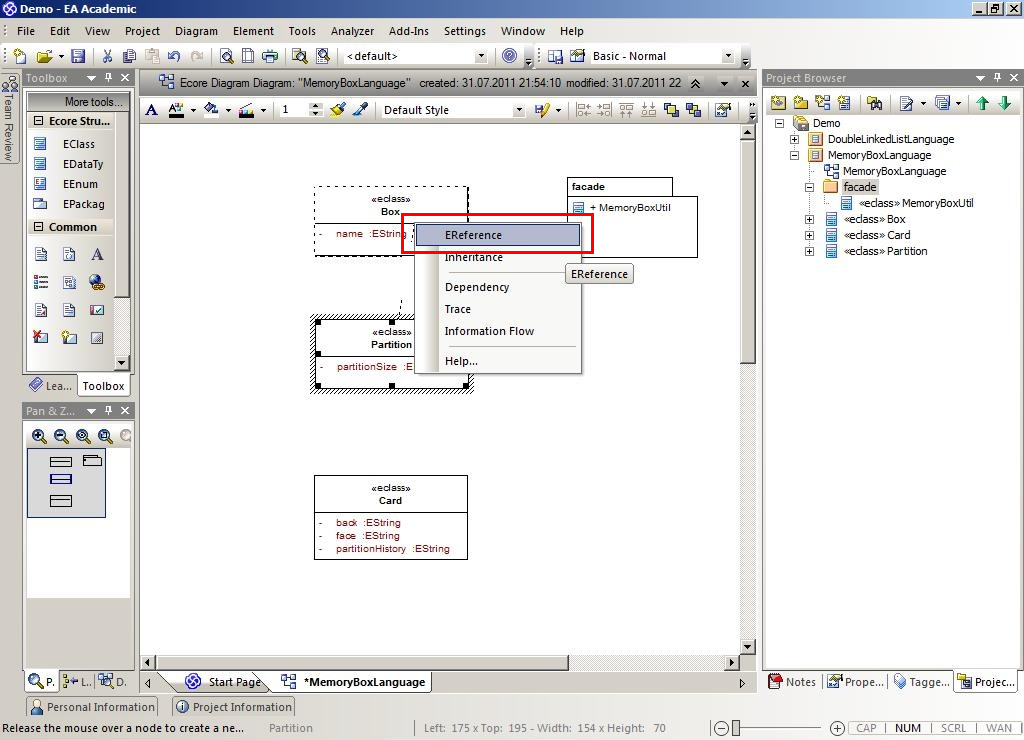
\includegraphics[width=0.6\textwidth]{pics/memBox24.png}
	\caption{Create a reference via Quick Link.}
	\label{fig:ereference}
\end{figure}

In the dialogue that pops-up (Fig.~\ref{fig:ereference_properties}), the
direction of the reference can be set.  The default is bidirectional and this is
ok for our \texttt{Box}-\texttt{Partition} connection.  A \texttt{Name} can also
be entered, which is only used for documentation purposes and is not relevant
for codegeneration.

\begin{figure}[htbp]
	\centering
  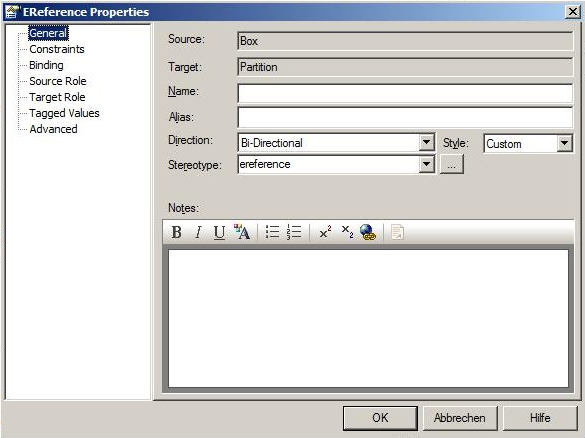
\includegraphics[width=0.6\textwidth]{pics/memBox25.png}
	\caption{Enter properties of the reference.}
	\label{fig:ereference_properties}
\end{figure}
	
\clearpage

In the same dialogue choose \texttt{Source Role} and enter the values in
Fig.~\ref{fig:ereference_properties} to set the properties for the ``source''
end of the reference (the \texttt{Box} role).  Important is a name for the role
(\texttt{box}), the \texttt{Multiplicity}, \texttt{Aggregation} and
\texttt{Navigability}.  Repeat the process for the \texttt{Target Role}.
  
\begin{figure}[htbp]
	\centering
  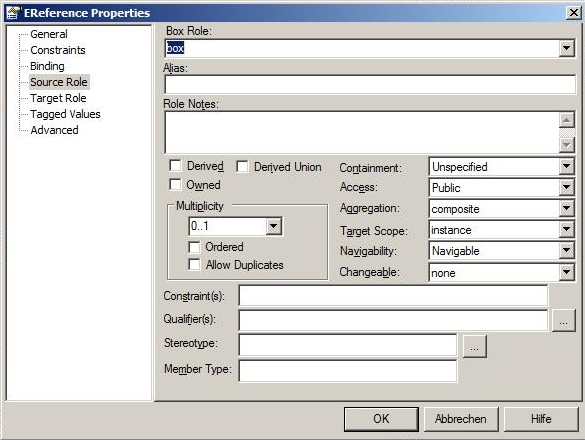
\includegraphics[width=0.5\textwidth]{pics/memBox26.png}\\
  \vspace{0.5cm}
  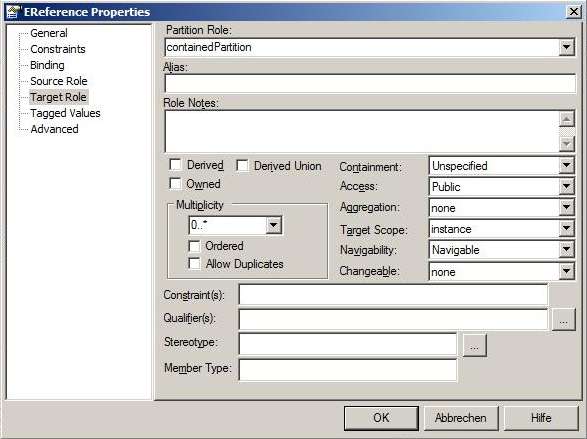
\includegraphics[width=0.5\textwidth]{pics/memBox27.png}
	\caption{Enter properties for source and target of reference.}
	\label{fig:reference_ends}
\end{figure}

Navigable ends are mapped to class attributes with getters and setters in Java
and therefore \emph{must} have a specified name and  multiplicity for successful
codegeneration.  
Corresponding Values for non-navigable ends can  be regarded as additional
documentation and do not have to be specified.
 
The multiplicity of a reference controls if the relation is mapped to a Java
Collection (\texttt{*},  \texttt{1..*}, \texttt{0..*}), or a single valued class
attribute (\texttt{1}, \texttt{0..1}).

In Ecore, the aggregation values of a reference can either be \texttt{none} or
\texttt{com\-po\-site}.  Composite means that the current role is that of a
\emph{container} for the opposite role.  In our case for example, \texttt{box}
is a container for \texttt{partitions}.\\  This has a series of
consequences: (1) every element must have a container, (2) an element cannot be
in more than one container at the same time, and (3) a container's contents are
deleted together with the container.  Non-composite (\texttt{none}) means that
the current role is not that of a container and the rules for containment do not
hold (reference is a simple ``pointer'').

\clearpage

If you've done everything right, your workspace should now resemble
Fig.~\ref{fig:ereference_completed} with a relation between \texttt{Box} and
\texttt{Partition}.

\begin{figure}[htbp]
	\centering
  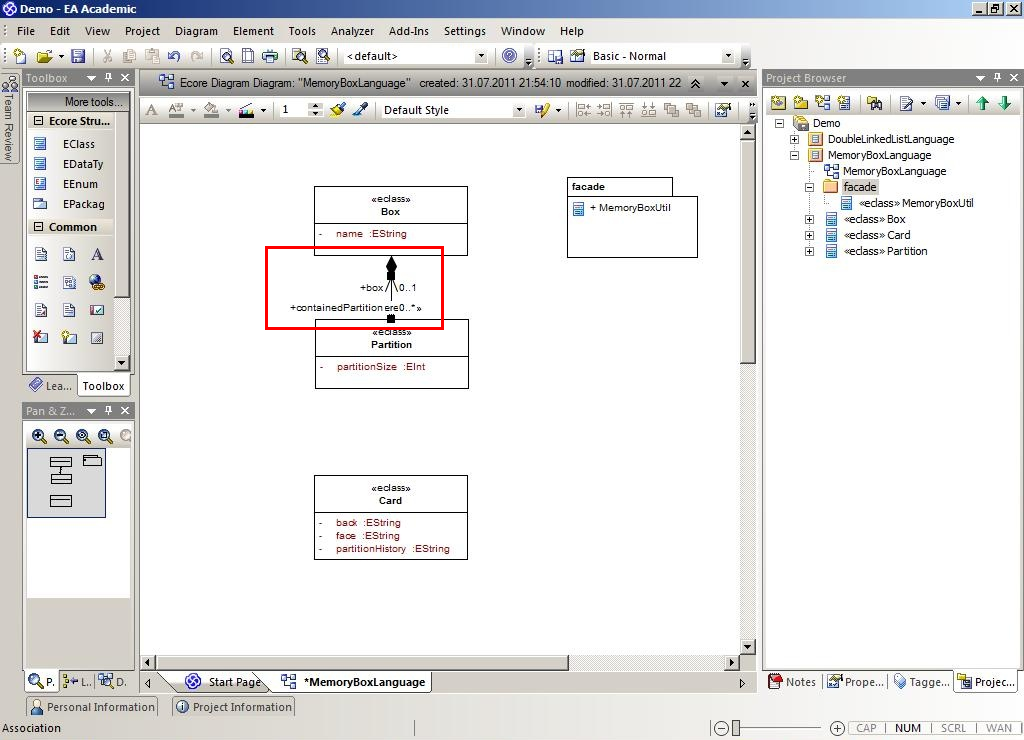
\includegraphics[width=0.7\textwidth]{pics/memBox28.png}
	\caption{\texttt{Box} contains \texttt{Partition}s.}
	\label{fig:ereference_completed}
\end{figure}

Create a bidirectional reference\footnote{To be precise, \emph{all} references
in Ecore are actually unidirectional.  A ``bidirectional'' reference in our
metamodel is in reality mapped to two \texttt{EReferences} that are opposites of
each other.  
We however believe it is simpler to handle these pairs as single references and
prefer this concise concrete syntax.} between \texttt{Partition} and \texttt{Card}
and two unidirectional self-references for \texttt{Partition} according to
Fig.~\ref{fig:ereferences_all}.
 
\begin{figure}[htbp]
	\centering
  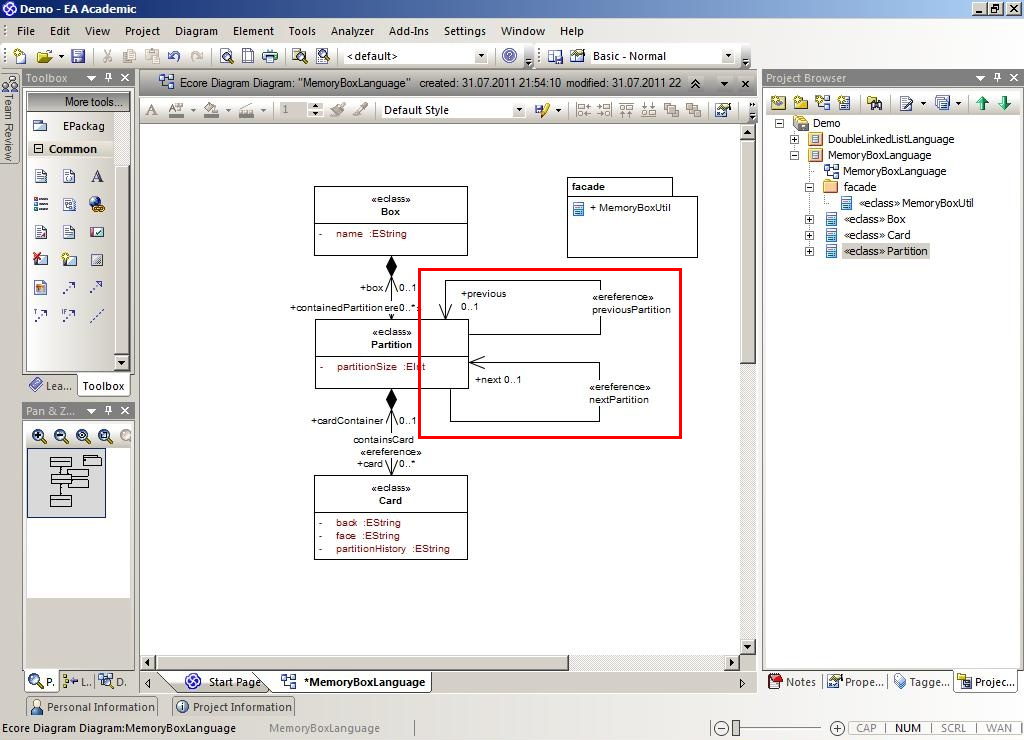
\includegraphics[width=0.7\textwidth]{pics/memBox34.png}
	\caption{All relations in our metamodel.}
	\label{fig:ereferences_all}
\end{figure}

\clearpage

Every system has, in addition to its static structure, certain dynamic aspects
that describe the system's behaviour and how it evolves over time or reacts to
external stimulus.
\marginpar{\emph{Dynamic Semantics}}
In a language, these rules that govern the dynamic behaviour of a system are
referred to collectively as the \emph{Dynamic Semantics} of the language.  
Although these rules can be defined as a set of separate \emph{Model
Transformations}, we take a holistic approach and advocate integrating the
transformations directly in the metamodel as operations.
This fits nicely to the object oriented paradigm and is quite natural in many
cases.  In the next few steps we shall define the \emph{signatures} of some
operations for our memory box.  We will of course use SDMs to \emph{implement}
the methods later.

Right-click \texttt{Partition} to invoke the context-menu depicted in
Fig.~\ref{fig:add_operation} and choose \texttt{Operations\ldots}.

\begin{figure}[htbp]
	\centering
  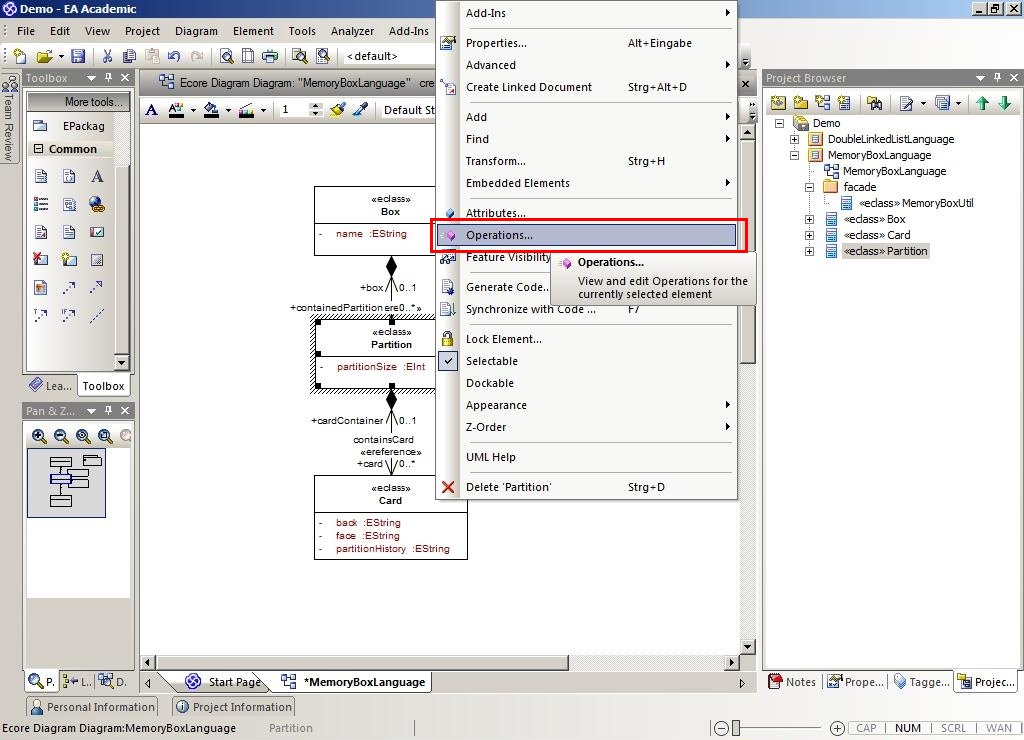
\includegraphics[width=0.6\textwidth]{pics/memBox35.png}
	\caption{Add an operation.}
	\label{fig:add_operation}
\end{figure}
 
In the dialogue that pops-up (Fig.~\ref{fig:operation_properties}), enter
\texttt{empty} as the \texttt{Name} of the operation, leave the \texttt{Return
Type} as \texttt{void}.  Press \texttt{Save}.
 
\begin{figure}[htbp]
	\centering
  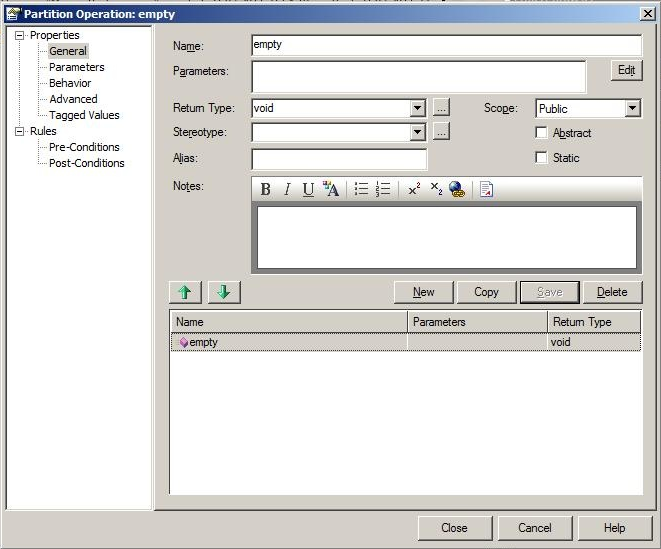
\includegraphics[width=0.45\textwidth]{pics/memBox37.png}
	\caption{Properties for operation.}
	\label{fig:operation_properties}
\end{figure}

\clearpage

In the same dialogue, press \texttt{New} to add further operations and enter the
values in Fig.~\ref{fig:operation_parameters}.  Parameters can be added by
pressing \texttt{Edit} and entering the name and choosing the type of each
Parameter in a separate dialogue.

\begin{figure}[htbp]
	\centering
  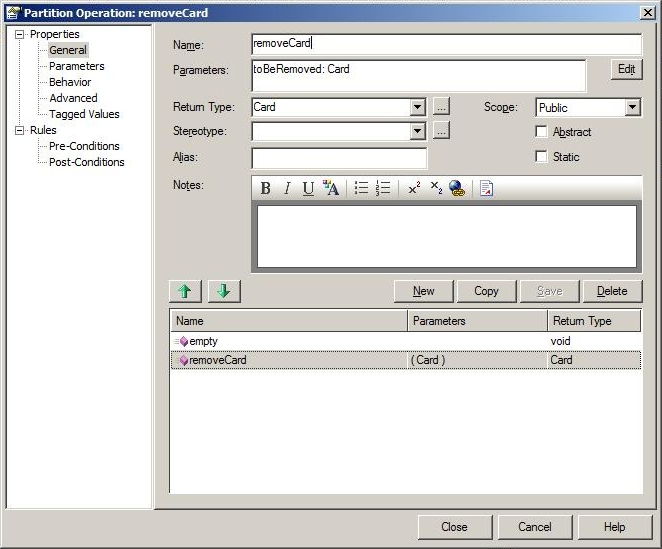
\includegraphics[width=0.6\textwidth]{pics/memBox38.png}
	\caption{Parameters and Return Type.}
	\label{fig:operation_parameters}
\end{figure}

Repeat the process for the values in Fig.~\ref{fig:operation_partition}.  The
\texttt{Return Type} can be chosen via the drop-down menu for primitives
(\texttt{EBoolean}), or via the \texttt{\ldots} button for types in the
metamodel (\texttt{Card}). 

If you've done everything right, your dialogue should
now contain three methods \texttt{check}, \texttt{empty}, and
\texttt{removeCard} with corresponding parameters and return types as in
Fig.~\ref{fig:operation_partition}.

\begin{figure}[htbp]
	\centering
  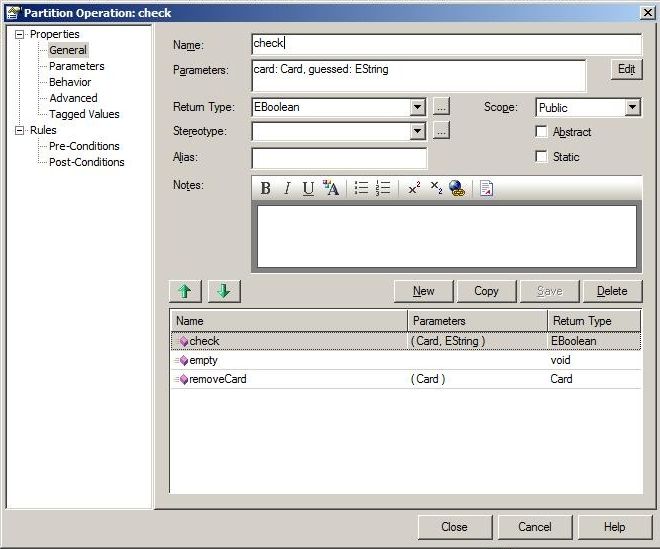
\includegraphics[width=0.6\textwidth]{pics/memBox39}
	\caption{All operations in \texttt{Partition}.}
	\label{fig:operation_partition}
\end{figure}

\clearpage

Add all operations analogously for \texttt{Box} and \texttt{Card} so that your
metamodel closely resembles Fig.~\ref{fig:metamodel_complete}.
 
\begin{figure}[htbp]
	\centering 
  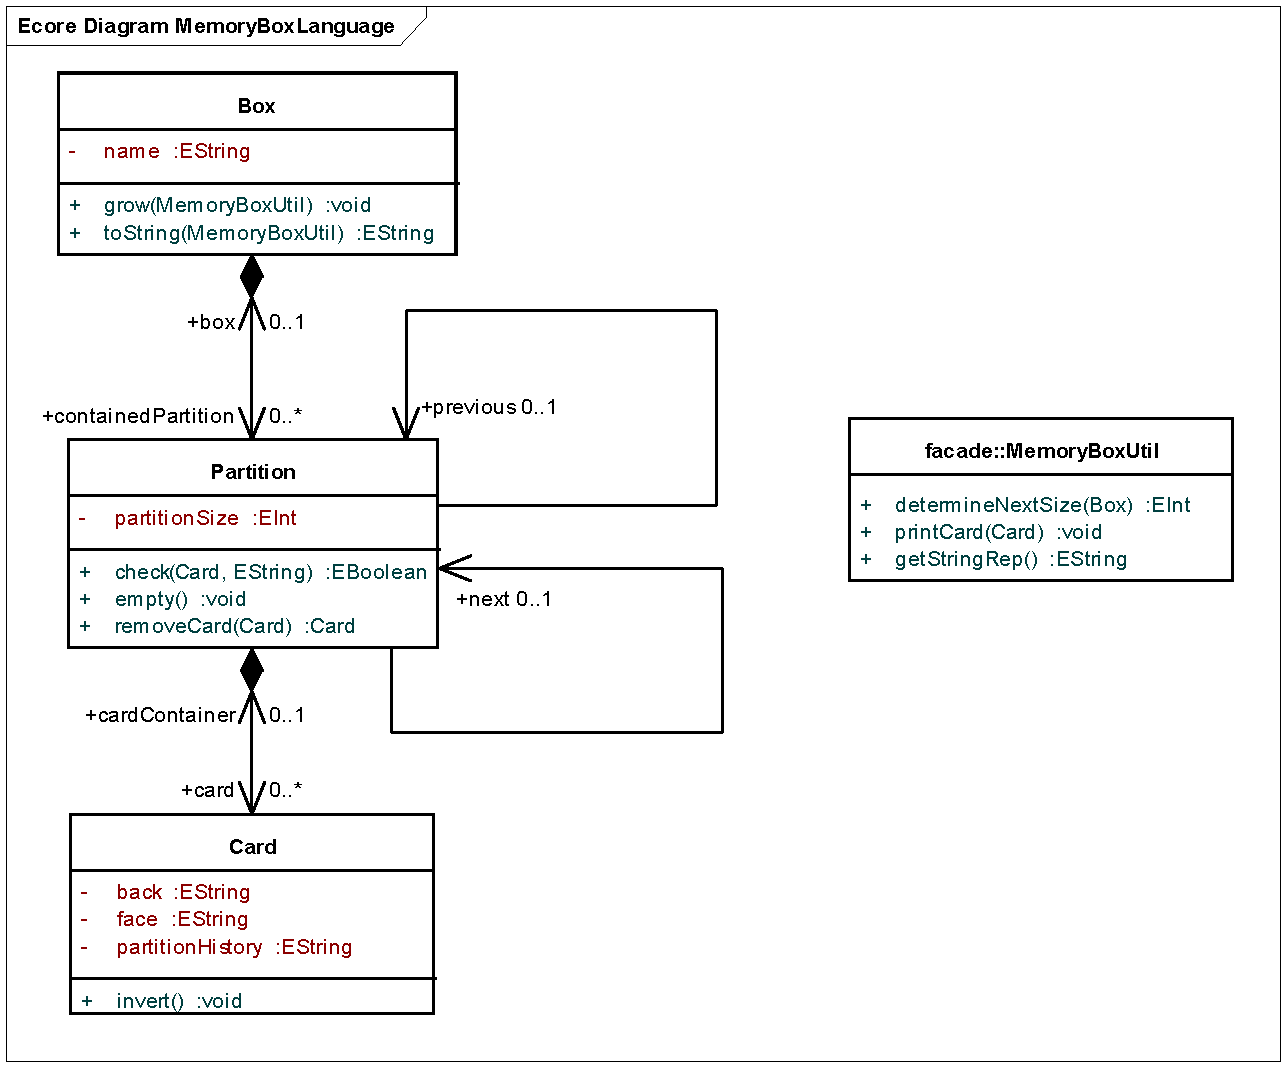
\includegraphics[width=\textwidth]{pics/memBox44} 
	\caption{Complete metamodel for our memory box.}
	\label{fig:metamodel_complete}
\end{figure}

Lets take a step back and review our metamodel.  We have modelled a \texttt{Box}
that contains arbitrary many \texttt{Partition}s.  A \texttt{Partition} in the
\texttt{Box} has a \texttt{next} and \texttt{previous} \texttt{Partition} that
can be set or not. Finally, \texttt{Partition}s contain \texttt{Card}s.

A \texttt{Box} has a \texttt{name}, and can be extended by calling
\texttt{grow}. A \texttt{Box} can print out its contents via \texttt{toString}. 
We'll see later in the tutorial why these two methods need our
\texttt{MemoryBoxUtil} as a parameter.

The main method of the memory box is \texttt{Partition::check} that takes a
\texttt{Card} and the user's guess as an \texttt{EString} and returns
\texttt{true} or \texttt{false} depending on if the guess was correct or not.
A \texttt{Partition} can also \texttt{empty} itself of all \texttt{Cards}, or
\texttt{remove} a particular \texttt{Card}.  Last but not least, a
\texttt{Partition} has a \texttt{partitionSize} that can be used to indicate
that the \texttt{Partition} is full and is ready to be revised.

\clearpage

A \texttt{Card} contains the actual content to be learnt as a question on the
card's \texttt{face} and the answer on the card's \texttt{back}. A \texttt{Card}
also maintains a \texttt{partition\-History} which can be used to keep track of
how often a \texttt{Card} has been answered correctly/wrongly.  This might
indicate how difficult the \texttt{Card} is for a specific user.
When learning a language, it makes sense to be able to swap the target and
source langauge and this is supported by \texttt{Card} via \texttt{invert}
(turns the card around).

Now try to export the metamodel for codegeneration in Eclipse.  To do this
right-click on \texttt{MemoryBoxLanguage} and choose ``Add-In/MOFLON::Ecore
Addin/Export Selection to Workspace''.  Then switch to your Eclipse workspace
and refresh the metamodel workspace.

If you have done everything right, a new project \texttt{MemoryBoxLanguage}
should be created in the \texttt{Demo} working set in your Eclipse workspace.
If this is not the case please ensure that your metamodel is identical with
Fig.~\ref{fig:metamodel_complete}.  If you believe everything is correct and
things still don't work then feel free to contact us at
\url{contact@moflon.org}.  If code is generated successfully, take a look at all
the stuff that has been generated under \texttt{/gen}, especially the default
implementation for all methods that just throws an
\texttt{OperationNotSupported} exception.  We shall see later in the tutorial
that the EMF codegenerator actually supports merging hand-written
implementations of methods with generated code.  With eMoflon however, we can
also model a large part of the dynamic semantics and only need to implement
small helper methods for e.g. string manipulation by hand.

Let's move on and model the dynamic behaviour of our memory box!
\section{Dynamic Semantics with SDM}

The core idea when modelling behaviour is to regard dynamic aspects of a system
(let's call this a model as from now on) as bringing about a change of
state.
This means a model in state $S$ can evolve to state $S^*$ via a
transformation $\Delta: S \stackrel{\Delta}{\rightarrow}S^*$.
In this light, dynamic or behavioural aspects of a model are synonymous with
\emph{model transformations}, and the dynamic semantics of a language equate
simply to a suitable set of model transformations.
This approach is once again quite similar to OO where objects have state and can
\emph{do} things via methods that manipulate their state.        

So how do we model model transformations?  There are quite a few possibilities.
We could employ a suitably concise imperative programming language with which we
simply say in a step-by-step manner how the system morphs.
There actually exist quite a few very successful languages and tools in this
direction.

But isn't this almost like just programming directly in Java?
There must be a better way to do this\ldots  From the relatively mature
area of graph grammars and graph transformations we take a \emph{declarative}
and \emph{rule-based} approach.  
Declarative in this context means that we do not want to specify exactly how and
in what order changes to the model must be carried out to achieve a
transformation. 
We just want to say under what conditions the transformation can be executed
(precondition), and the state of the model after executing the transformation
(post condition). 
The actual task of going from precondition to postcondition should  be taken
over by a transformation engine and all related details are basically regarded
as a black box.         

Ok - so a model transformation is of the form $(pre, post)$.  Inspired by string 
grammars, let's call this black box transformation a \emph{rule}, and
consequently the precondition the left-hand side of the rule $L$ and the
postcondition the right-hand side $R$.  

A rule $r: (L,R)$ can be \emph{applied} to a model (a typed graph) $G$ by:
\begin{enumerate}
  \item Finding an occurrence of the precondition $L$ in $G$ via a \emph{match}
  $m$,
  \item Cutting out $Destroy := (L\setminus R)$ i.e., the elements that are
  present in the precondition but not in the postcondition are to be deleted,
  from $G$ to form  $(G\setminus Destroy)$ and
  \item Pasting $Create := (R\setminus L)$ i.e., new elements that are
  present in the postcondition but not in the precondition and are to be
  created, into the hole in $(G\setminus Destroy)$ to form a new graph $H =
  (G\setminus Destroy) \cup Create$.
\end{enumerate}

Rule application is denoted as $G \stackrel{r}{\Rightarrow} H$ and is depicted
in Fig.~\ref{fig:rule_application}. 

%\usepackage{graphics} is needed for \includegraphics
\begin{figure}[htp]
\begin{center}
  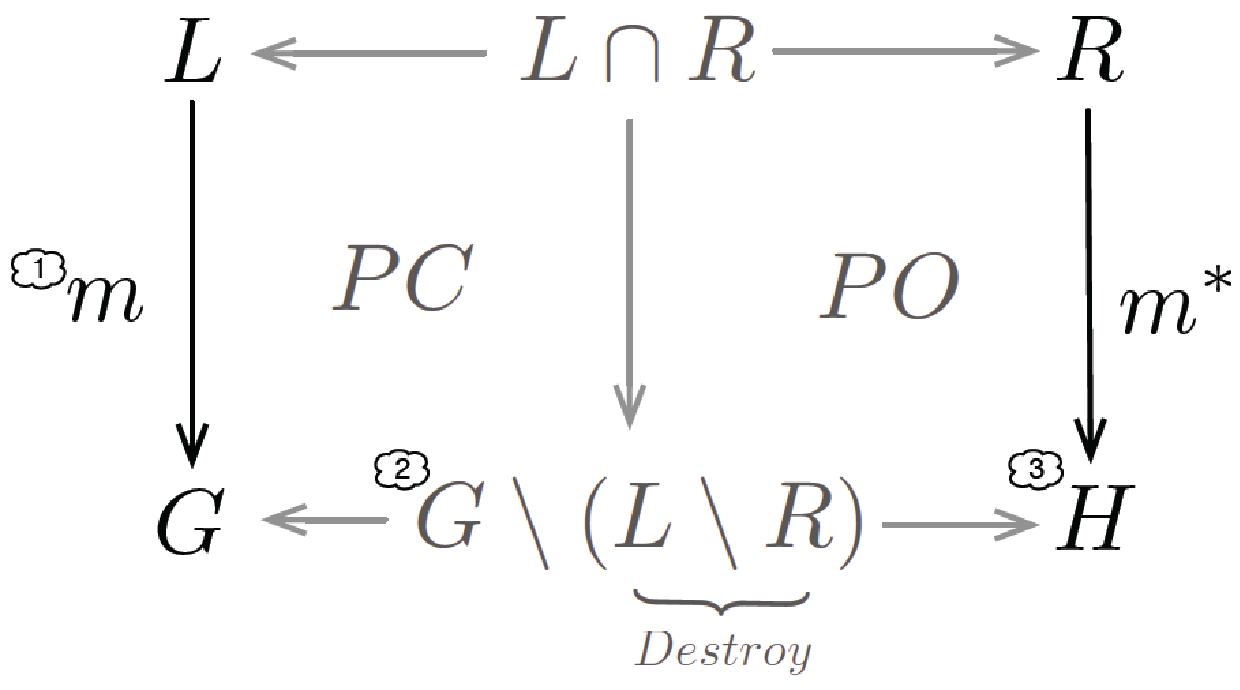
\includegraphics[width=0.6\textwidth]{pics/rule_application}
  \caption[]{Applying a rule $r: (L,R)$ to $G$ to yield $H$} 
  \label{fig:rule_application}
\end{center}
\end{figure}

(1) is called \emph{graph pattern matching}, (2) is called building a
\emph{push-out complement} $PC = (G\setminus Destroy)$, so that $L \cup
(G\setminus Destroy) = G$ and (3) is called building a \emph{push-out} $PO = H$,
so that $(G\setminus Destroy) \cup R = H$. A push-out is a generalised union
defined on typed graphs.  As we are dealing with graphs here, it is not such a
trivial task to define (1) -- (3) in precise terms with conditions when a rule
can be applied and not, and there exists substantial theory with exactly that
goal. As this formalisation of rule application involves two push-outs: one
(deletion) when cutting out $Destroy := (L\setminus R)$ from $G$ to yield
$(G\setminus Destroy)$, and one (creation) when inserting $Create := (R\setminus
L)$ in $(G\setminus Destroy)$ to yield $H$, this is referred to as a
\emph{double push-out}.  
We won't go into further details in this tutorial, but the interested reader can
refer to [Ref] for the exciting details.  

Now that we know what rules are, let's take a look at a simple example for our
memory box. How would a rule look like for moving a card from one partition to
the next?  Fig.~\ref{fig:rule_example} depicts the rule $moveCard$.
  
%\usepackage{graphics} is needed for \includegraphics
\begin{figure}[htp]
\begin{center}
  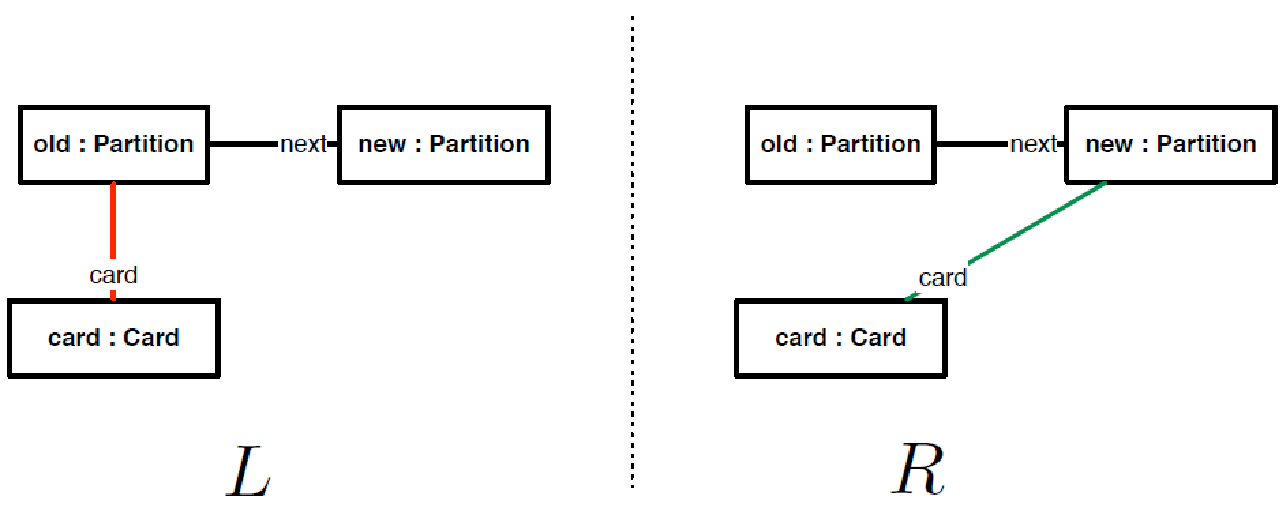
\includegraphics[width=0.9\textwidth]{pics/rule_example}
  \caption[]{Rule $moveCard$ as a graph transformation rule.}	
  \label{fig:rule_example}
\end{center}
\end{figure}

\clearpage

As already indicated by the colours used for $moveCard$ we employ a compact
representation of rules that is formed by merging $(L,R)$ into a single
\emph{story pattern} composed of  $Destroy := (L\setminus R)$ in red, $Retain := 
L\cap R$ in black, and $Create := (R\setminus L)$ in  green
(Fig.~\ref{fig:rule_compact}).
%\usepackage{graphics} is needed for \includegraphics
\begin{figure}[htp]
\begin{center}
  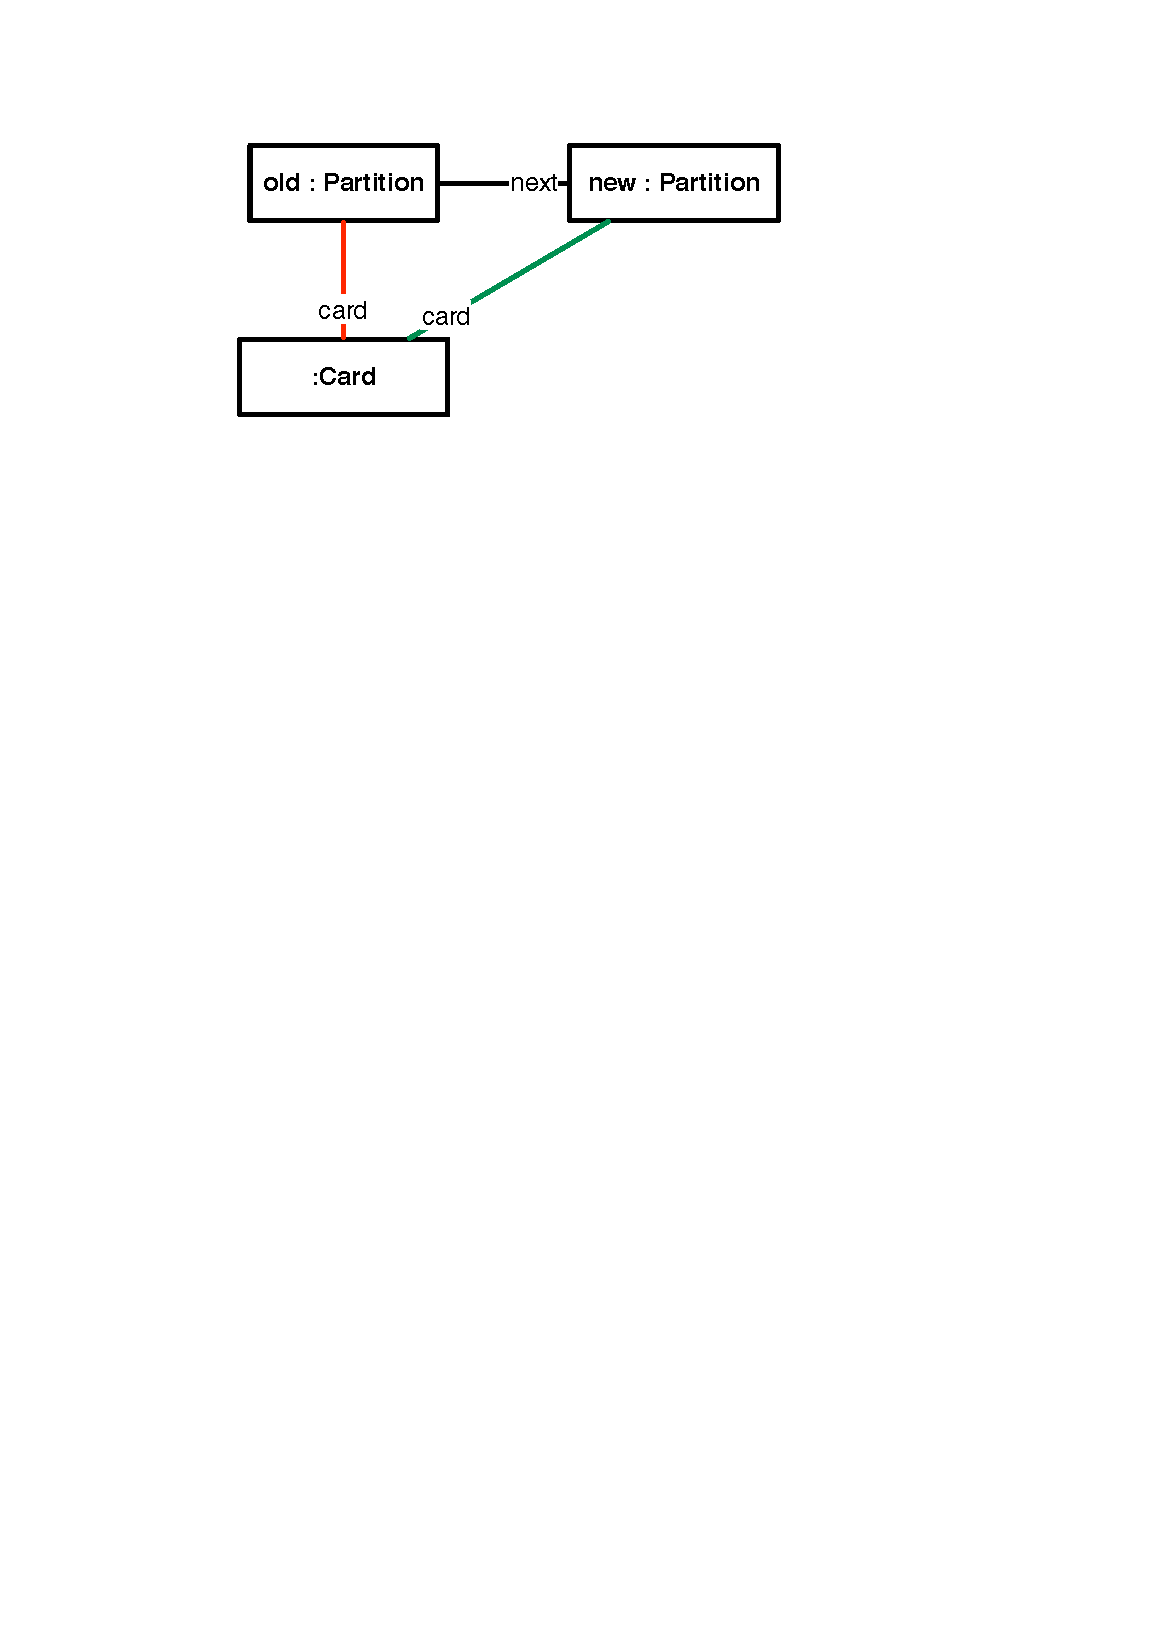
\includegraphics[width=0.45\textwidth]{pics/rule_compact}
  \caption[]{Compact representation of $moveCard$ as a Story Pattern.}
  \label{fig:rule_compact}
\end{center}
\end{figure}

 As we shall see in a moment, this  representation is quite intuitive and one can
just forget the details of rule application and think in terms of what is to be
deleted, retained and created. Applying $moveCard$ to a memory box according to
steps (1) -- (3) is depicted in Fig.~\ref{fig:rule_app_example}.

%\usepackage{graphics} is needed for \includegraphics
\begin{figure}[htp] 
\begin{center}
  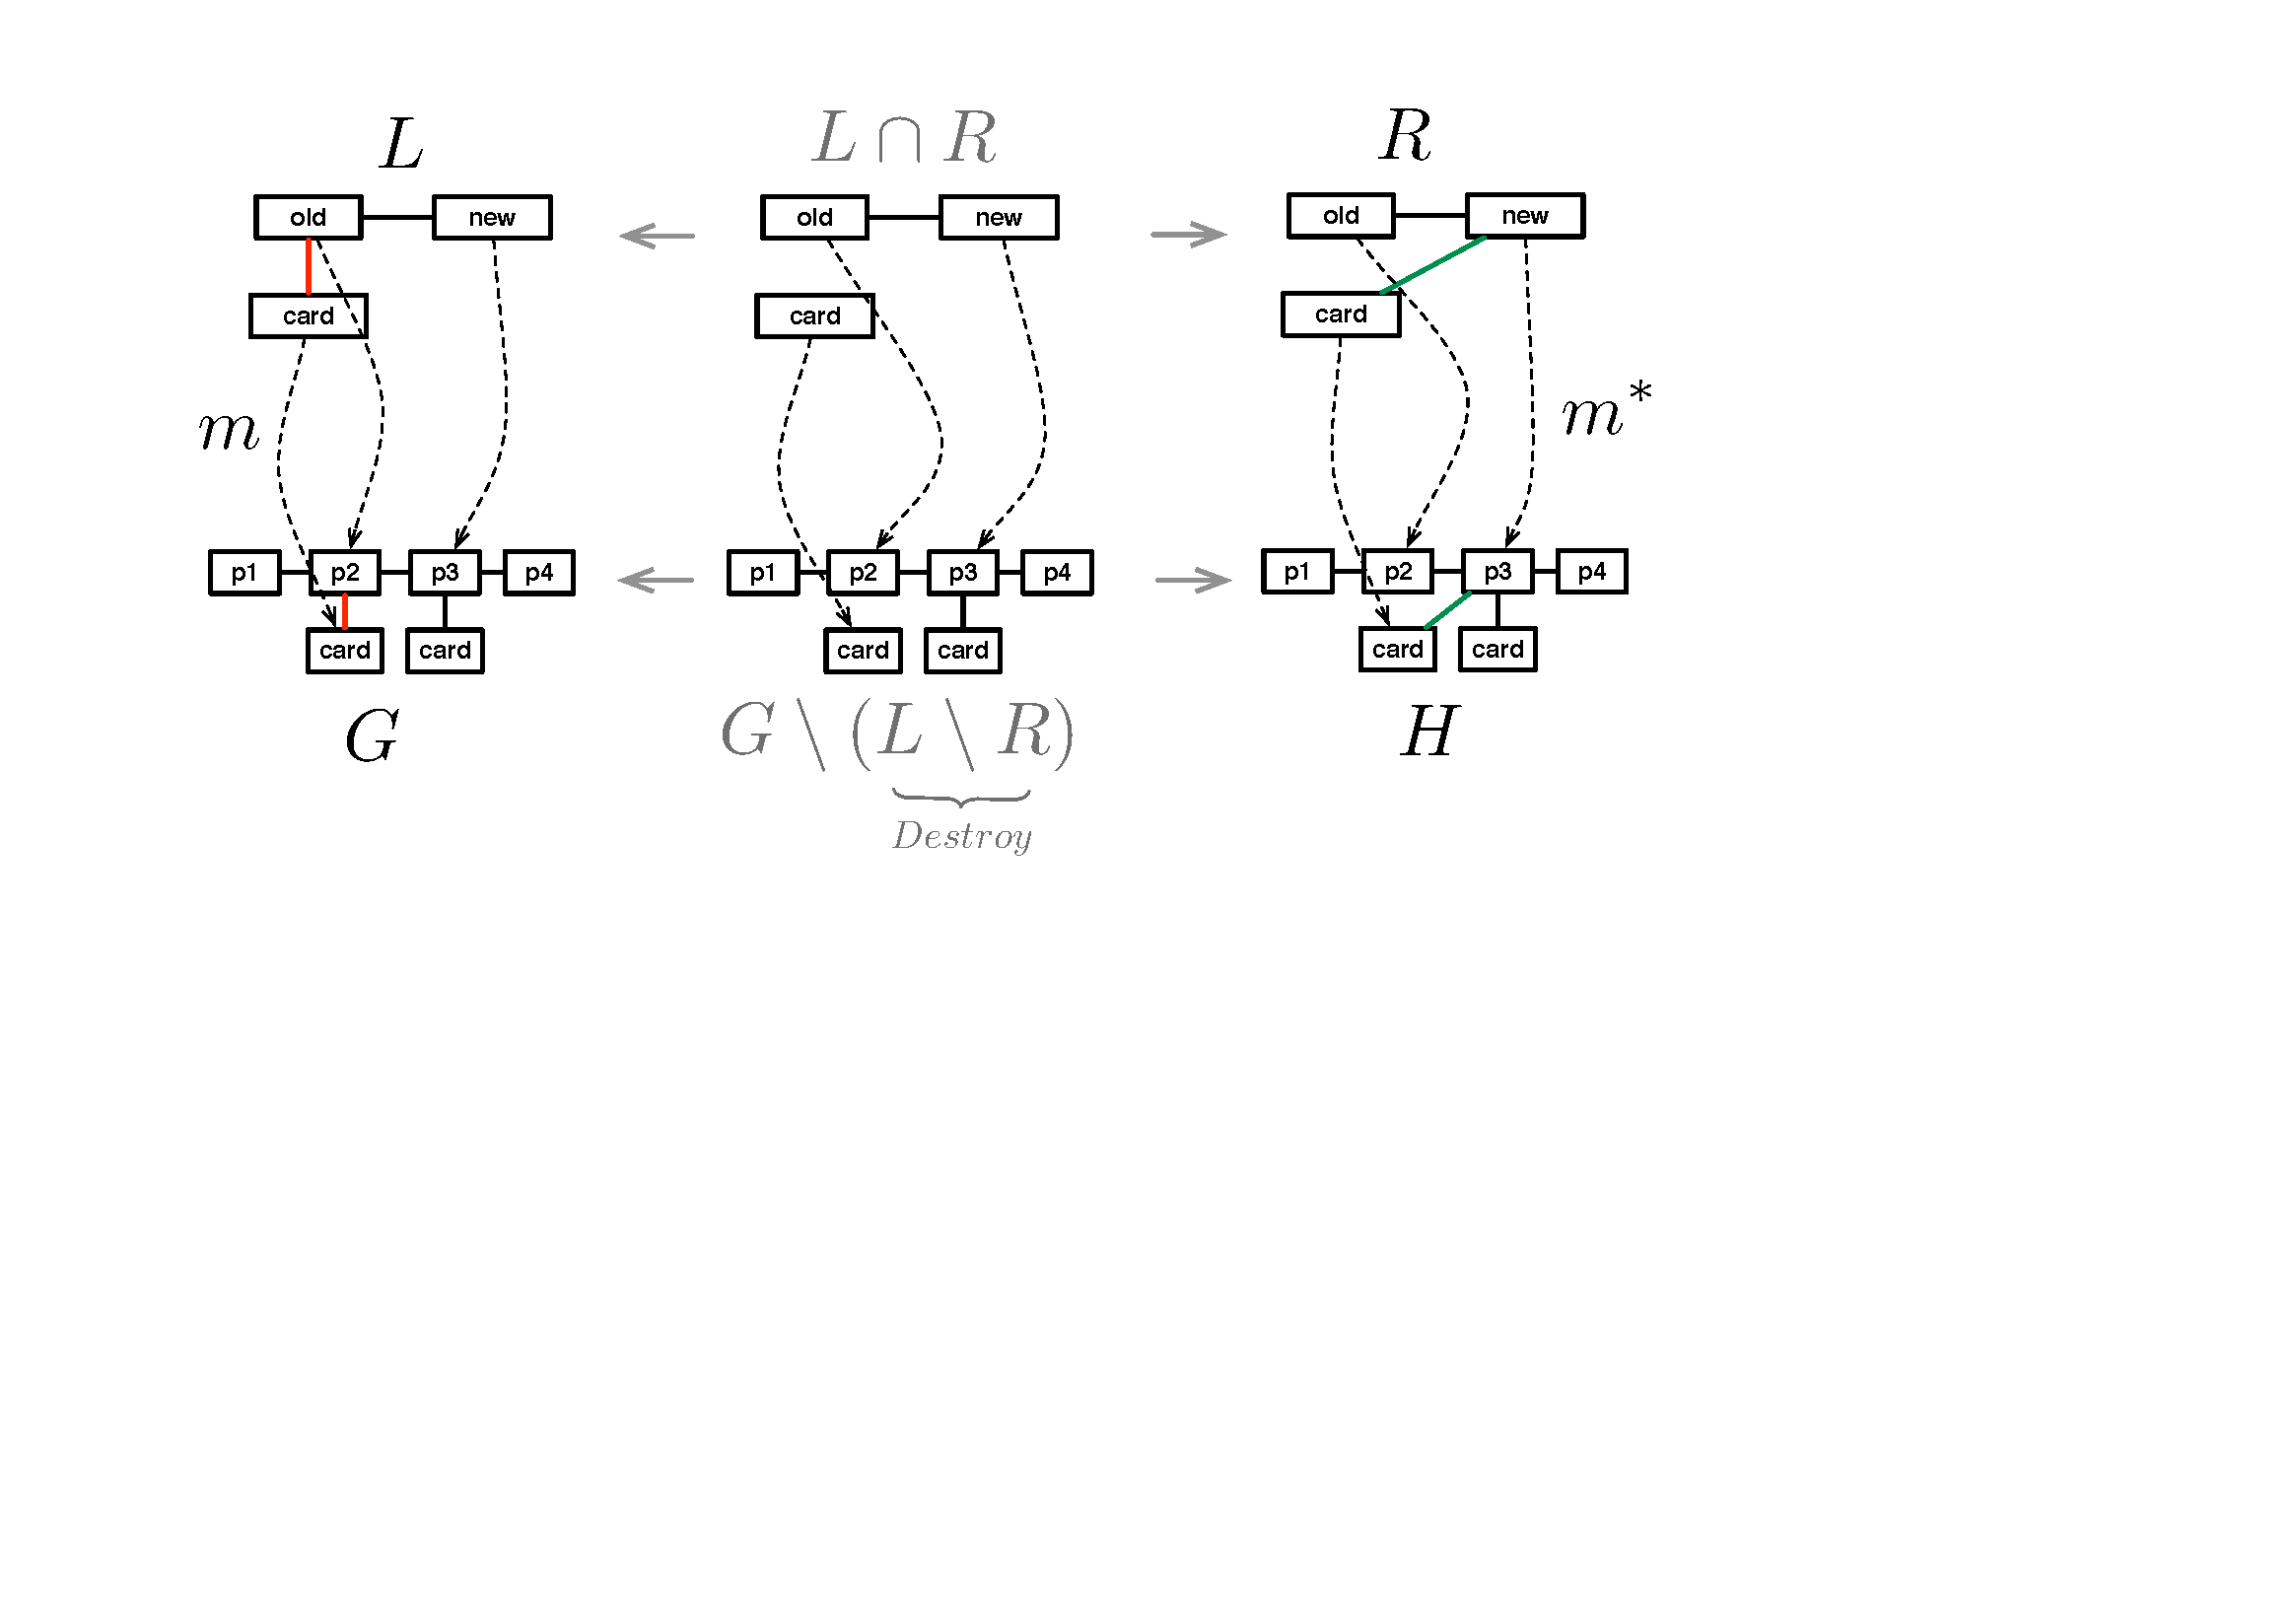
\includegraphics[width=\textwidth]{pics/rule_app_example}
  \caption[]{Applying $moveCard$ to a memory box.}
  \label{fig:rule_app_example}
\end{center}
\end{figure}

\clearpage 

One last thing before we continue with our memory box; individual rules still
have to be applied in a suitable sequence to realise complex model
transformations that consist of many steps.  This is realised with simplified
activity diagrams, where a single activity node is a pattern as discussed above,
and activity edges join nodes to form a control flow.   This can be viewed as
two layers:  an imperative layer to define the top-level control flow via
activity diagrams (if-else statements, loops etc), and a pattern layer
consisting of a story pattern in each activity node that specifies, via a graph
transformation rule, how the model is to be manipulated in that step.         

Enough theory! Grab your mouse and let's get cracking with SDMs\ldots

\end{document}